\documentclass{article}

\usepackage[margin=0.7in]{geometry}
\usepackage[parfill]{parskip}
\usepackage[utf8]{inputenc}

\usepackage{graphicx} % For including images
\graphicspath{ {./images/} }
\usepackage{subcaption} % For subfigures
\usepackage[table]{xcolor} % For alternate coloring in tables

\usepackage{amsmath,amssymb,amsfonts,amsthm} % Math packages

\usepackage{cleveref} % Inline referencing
\usepackage[style=alphabetic]{biblatex} % For bibliography
\addbibresource{bibliography.bib}

\usepackage{setspace} % For double-spacing
\doublespacing

% Some macros
\newcommand\solmass{\textrm{M}_\odot}
\newcommand\kpc{\textrm{kpc}}
\newcommand\kmps{\textrm{km}/\textrm{s}}

\newcommand\vrot{\ensuremath{v_{\textrm{rot}}}}
\newcommand\vobs{\ensuremath{v_{\textrm{obs}}}}

\title{Mass Distributions of Spiral Galaxies}
\date{}

\begin{document}

\maketitle

\section{Introduction}\label{sec:introduction}

The astronomer Edwin Hubble, in a series of lectures given at Yale in 1935\footnote{These lectures were later published under the title \textit{The Realm of the Nebulae} \cite{Hubble1936}.}, provided a classification of galaxies, which he refered to as \textit{extragalactic nebulae}, into spiral and elliptic.
This classification is used even today by amateur and professional astronomers alike, though the expanded version provided by French astronomer Gérard de Vaucouleurs is preferable.
But nowadays, the morphological classification of galaxies --- classifying galaxies based on what we perceive their shape to be --- is done computationally.

\begin{figure}[h!]
    \centering
    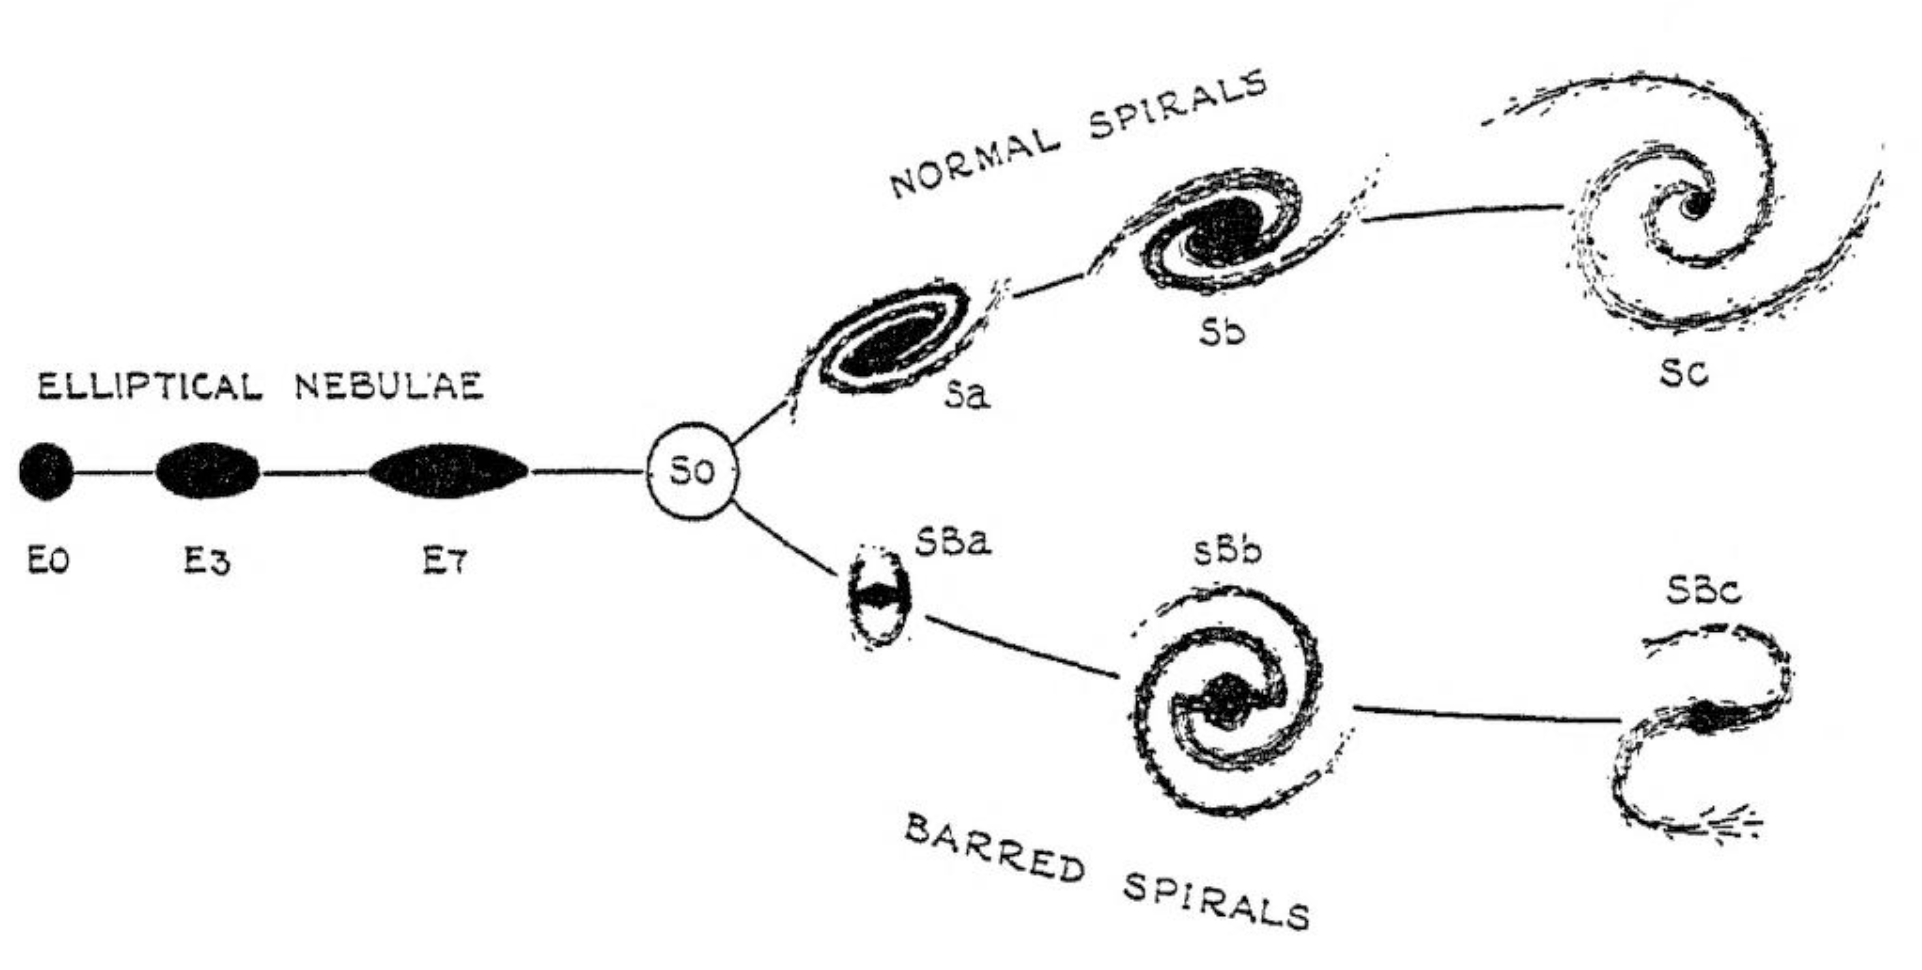
\includegraphics[width=0.7\linewidth]{hubblefork}
    \caption{Hubble's "tuning fork" classification scheme, p. 45, \cite{Hubble1936}.}
    \label{fig:hubblefork}
\end{figure}

What has enabled such computational work is the signficant progress in our ability to make precise astronomical observations over large distances and use them to make physical deductions.
One specific instance of this is the use of spectroscopy to understand the motion of galaxies relative to us, in which one measures at two seperate occassions the electromagnetic spectrum radiated by a galaxy using a \textit{spectrometer} and uses the shift observed in the emission lines to calculate the speed at which the galaxy is moving relative to us.
By making this measurement at different distances from the center of a galaxy, under the assumption that a galaxy is centrally symmetric, and accounting for the inclination possessed by the galaxy when we observe it, we can plot the \textit{rotation curve} of a galaxy; a plot of the rotational velocity against the galactocentric radius.

Since the velocity of a body in circular motion can be related to its mass using Newton's second law, I therefore explore the rotation curves of spiral galaxies under the following research question:

\begin{center}
    \textit{How is the gravitational mass of a spiral galaxy distributed within its disc, and how is this distribution determined by the rotational velocities?}
\end{center}

% \begin{itemize}
%     \item What are spiral galaxies?
%     \item Edwin Hubble's work.
%     \item What measurements have been made about spiral galaxies?
%     \item Go relatively deep; show that you've done reading outside of IB.
%     \item RQ: How is the gravitational mass of a spiral galaxy distributed within its disc, and how is this distribution determined by the rotational velocity distribution within and outside the disc?
% \end{itemize}

\section{Theory}\label{sec:theory}

Consider a spherical gas cloud of radius \(R\) and uniform density \(\rho\) that is rotating about its centre.
The rotational speed \(v_{\text{rot}}\) of a particle of mass \(m\) at distance \(r\) from the centre can be found using Newton's law of gravitation and second law of motion, which give us
\[\frac{mv_{\text{rot}}^2}{r} = \frac{GmM}{r^2},\]
or simply

\begin{equation}
    v_{\text{rot}} = \sqrt{GM/r},
    \label{eq:vrotcummass}
\end{equation}

where \(M\) is the mass of the cloud internal to the particle, naturally called the \textit{cumulative mass of the galaxy}.
Substituting

\begin{equation}\label{eq:massdense}
    M =
    \begin{cases}
        \frac{4}{3}\rho\pi r^3 & (r < R) \\
        \frac{4}{4}\rho\pi R^3 & (r \ge R)
    \end{cases}
\end{equation}

into \Cref{eq:vrotcummass} gives

\begin{equation}\label{eq:vrotdense}
    \vrot = 
    \begin{cases}
        \sqrt{\frac{G\cdot \frac 4 3 \pi \rho r^3}{r}} = \sqrt{\frac{4\rho G\pi}{3}} r & (r < R) \\
        \sqrt{\frac{G\cdot \frac 4 3 \pi \rho R^3}{r}} = \sqrt{\frac{4\rho G\pi R^3}{3}} r^{-1/2} & (r \ge R)
    \end{cases}.
\end{equation}

So for a spiral galaxy that can be accurately modelled as a spherical gas cloud of uniform density, we can graph its expected rotation curve and cumulative mass distribution as described by \Cref{eq:massdense,eq:vrotdense}; see \Cref{fig:expectedgraphs}.
Note that in this paper we use astronomical units of measurement to ease our calculations: masses are in \textit{solar masses} (\(\solmass\)), distances are in \textit{kiloparsecs} (\(\kpc\)), and velocities and speeds are in \textit{kilometers per second} (\(\kmps\)).

\begin{figure}
    \centering
    \begin{subfigure}{0.4\textwidth}
        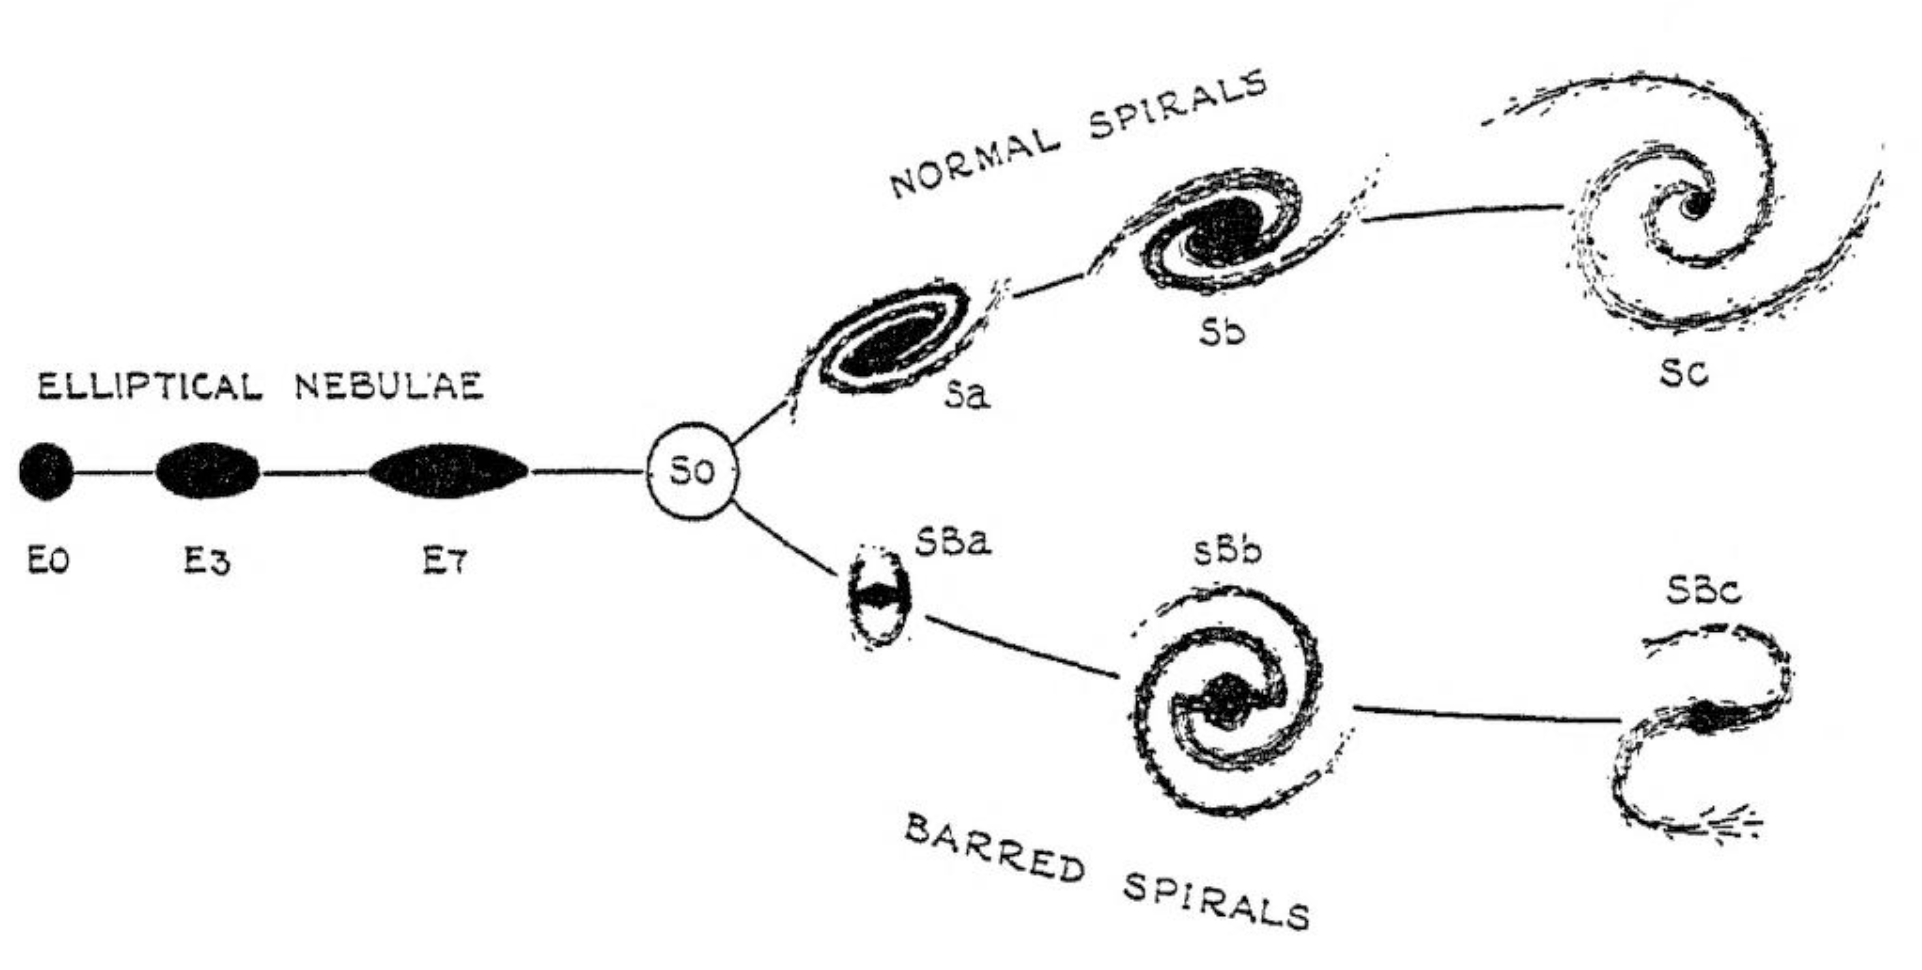
\includegraphics[width=\textwidth]{hubblefork}
        \caption{Rotation curve}
    \end{subfigure}
    \hfill
    \begin{subfigure}{0.4\textwidth}
        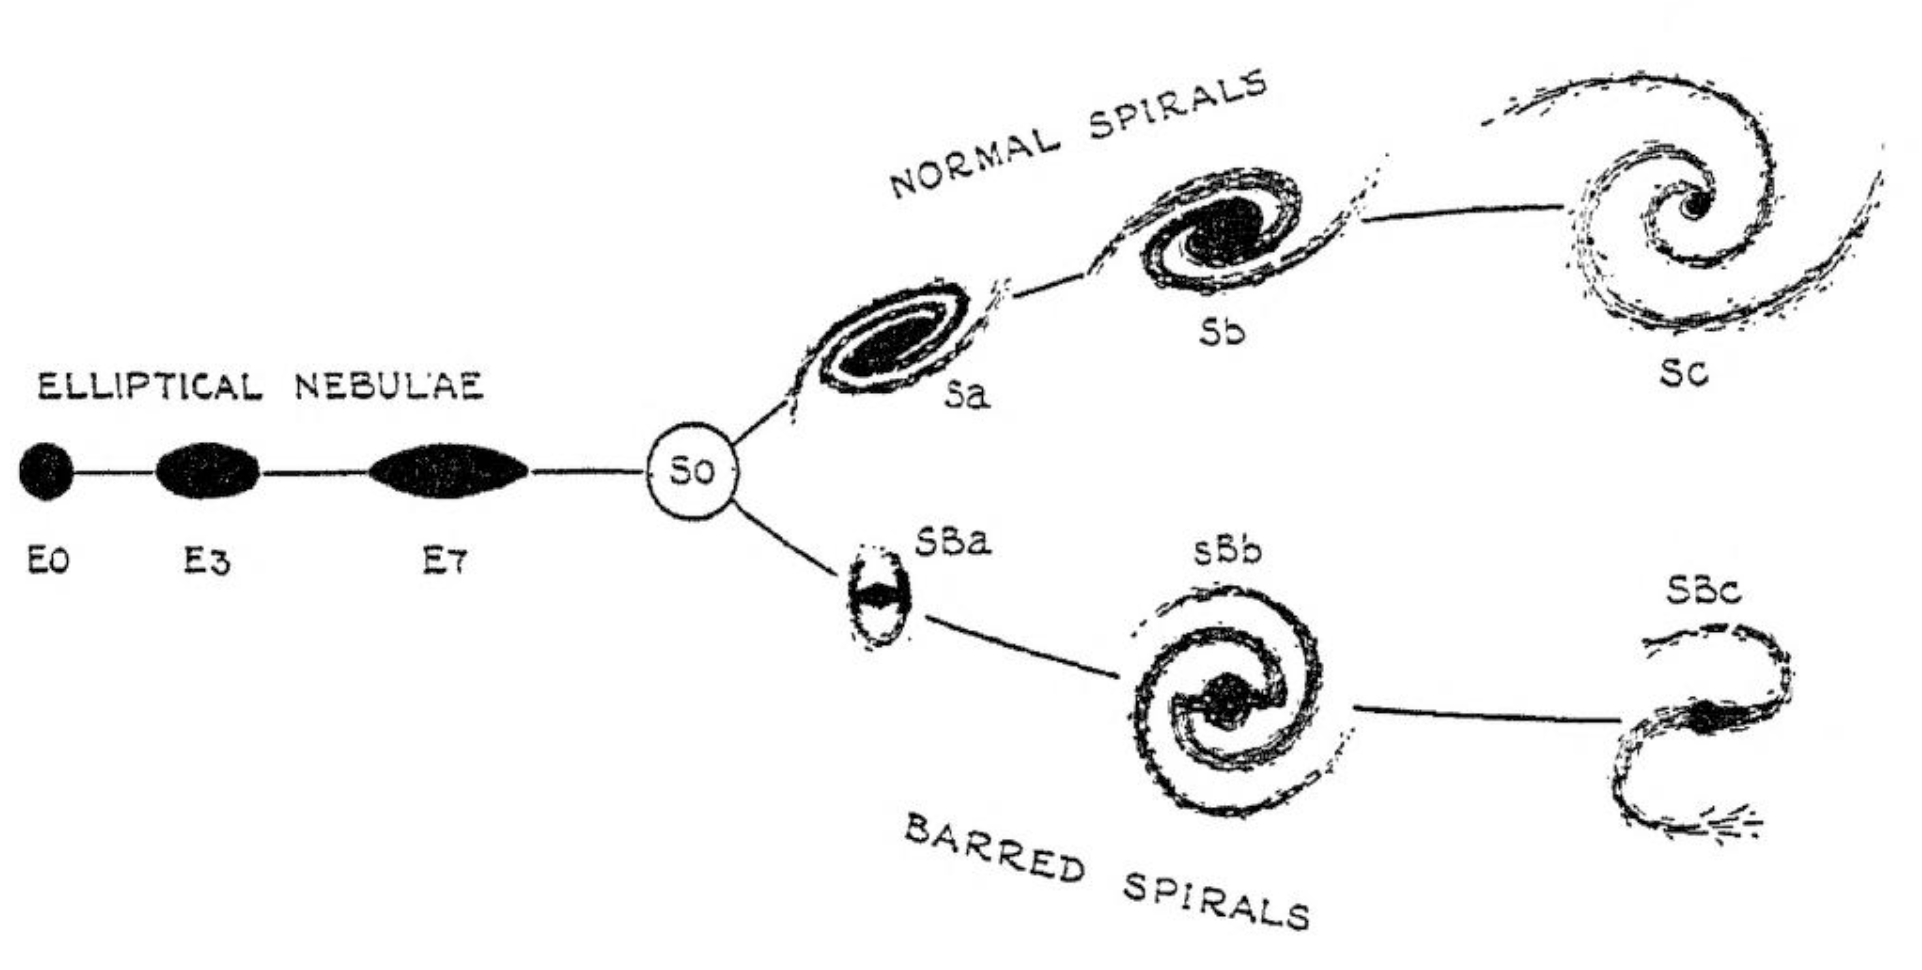
\includegraphics[width=\textwidth]{hubblefork}
        \caption{Cumulative mass distribution}
    \end{subfigure}
    \caption{Expected rotation curve and cumulative mass distribution for a galaxy.}
    \label{fig:expectedgraphs}
\end{figure}

However, as we shall see, the actual rotation curve of a spiral galaxy as well as the actual cumulative mass distribution does not look as in \Cref{fig:expectedgraphs}.

% \begin{itemize}
%     \item Number equations, to refer back to them.
%     \item Show the expected RC of a spiral galaxy.
%     \item Galaxies are usually moving away from us.
%     \item Don't say "galactocentric speed/velocity", rather "rotational speed/velocity".
% \end{itemize}

\section{Method}\label{sec:method}

This paper attempts to answer the proposed research question by analysing rotation curve data on the following galaxies: NGC0024, NGC0289, NGC1003, NGC2366, NGC2403.
The paper relies on two main sources for relevant data.
The observed velocities at various distances from the centres of these galaxies and the inclinations of the galaxies are taken from \Cite{SPARC}, which is a database of 175 spiral and irregular galaxies (including the ones mentioned above) using photometric and spectroscopic measurements from the Spitzer Space Telescope.
The chosen galaxies are all of them intentionally spiral galaxies, as the theory developed in \Cref{sec:theory} would not remain accurate for irregulars.
In addition to this database, the paper also makes use of the NASA/IPAC Extragalactic Database to ascertain the diameter of the visible disc of each of the chosen galaxies.

The paper is structured as follows.
The raw data required from the aforementioned databases is tabulated in \Cref{sec:raw-data}; this includes the radii and inclinations of the galaxies, as well as a table for each galaxy tabulating observed velocities at different distances from the centre.
Due to space requirements, this has been pushed to the appendix.
\Cref{sec:processed-data} uses this information to compute and plot the rotation curves and cumulative mass distributions of all of the galaxies.
These graphs are analysed in \Cref{sec:analysis}, and conclusions are presented in \Cref{sec:conclusion}.
Finally, \Cref{sec:evaluation} provides a brief evaluation of the uncertainties involved.

\section{Processed Data}\label{sec:processed-data}

% ---- move to METHOD

% On rearranging \Cref{eq:vrotcummass} we also find that
% 
% \begin{equation}\label{eq:internalmass}
%     M = \frac{rv_{\text{rot}}^2}{G},
% \end{equation}
% 
% allowing us to calculate the cumulative mass distribution of a galaxy, which satisfies these conditions, given its rotation curve.

% ----

\Cref{tab:raw0024-0289,tab:raw1003-2366,tab:raw2403} (in \Cref{sec:raw-data}) tabulate the observed velocities for each galaxy at various distances from their centres.
\textbf{HOWEVER...}
To correct for this error and to find \(\vrot\), we can use the following equation:
\begin{equation}\label{eq:vrotfromvobs}
    \vrot = \frac{\vobs}{\sin\theta}.
\end{equation}
Here \(\theta\) is the \textit{inclination} of the galaxy in question.
\textbf{THIS IS BECAUSE...}

Now we can rearrange \Cref{eq:vrotcummass} to get the internal mass \(M\) of the galaxy up to any radial distance \(r\):
\begin{equation}\label{eq:internalmass}
    M = \frac{r\vrot^2}{G}.
\end{equation}
This is the total mass of all matter in the galaxy up to a radius \(r\), as \(\vrot\) represents the orbital velocity at a distance \(r\) from the center.

\Cref{eq:vrotfromvobs,eq:internalmass} are used to generate \Cref{tab:proc0024-0289,tab:proc1003-2366,tab:proc2403}.
Since we are using astronomical units, the value of \(G\) taken in \Cref{eq:internalmass} is \(G = 4.3009 \times 10^{-6} \, \kpc \cdot (\kmps)^2 \cdot \solmass^{-1}\).
The uncertainties used are explained in \Cref{sec:evaluation}.
\Cref{fig:ngc0024,fig:ngc0289,fig:ngc1003,fig:ngc2366,fig:ngc2403} are subsequently rendered using these tables in Microsoft Excel 2011, the error bars representing the uncertainties in the corresponding variable.
Note that due to the small uncertainty in \(r\) as compared to \(\vrot\) and \(M\), the error bars for \(r\) are not visible.

\singlespacing
\begin{table}[h!]
    \begin{tabular}{|c|c|c|}
        \hline
        \multicolumn{3}{|c|}{NGC0024} \\
        \hline
        $r$ ($\kpc \pm 0.01 \,\kpc$) & $\vrot$ ($\kmps$) & $M$ ($\solmass$) \\
        \hline
        $0.21$ & $19.36 \pm 7.8$ & $1.83\times 10^{07} \pm 1.55\times 10^{07}$ \\
        $0.32$ & $34.49 \pm 10.8$ & $8.85\times 10^{07} \pm 5.80\times 10^{07}$ \\
        $0.43$ & $40.16 \pm 10.1$ & $1.61\times 10^{08} \pm 8.51\times 10^{07}$ \\
        $0.54$ & $51.18 \pm 10.8$ & $3.29\times 10^{08} \pm 1.45\times 10^{08}$ \\
        $0.64$ & $64.53 \pm 9.3$ & $6.20\times 10^{08} \pm 1.89\times 10^{08}$ \\
        $0.74$ & $70.54 \pm 12.5$ & $8.56\times 10^{08} \pm 3.14\times 10^{08}$ \\
        $0.85$ & $80.00 \pm 11.5$ & $1.26\times 10^{09} \pm 3.80\times 10^{08}$ \\
        $0.96$ & $85.00 \pm 9.8$ & $1.61\times 10^{09} \pm 3.88\times 10^{08}$ \\
        $1.07$ & $86.89 \pm 9.6$ & $1.88\times 10^{09} \pm 4.34\times 10^{08}$ \\
        $1.17$ & $89.56 \pm 9.1$ & $2.18\times 10^{09} \pm 4.64\times 10^{08}$ \\
        $1.28$ & $92.12 \pm 8.8$ & $2.53\times 10^{09} \pm 5.04\times 10^{08}$ \\
        $1.38$ & $95.24 \pm 9.7$ & $2.91\times 10^{09} \pm 6.12\times 10^{08}$ \\
        $1.48$ & $97.91 \pm 10.9$ & $3.30\times 10^{09} \pm 7.55\times 10^{08}$ \\
        $1.59$ & $102.4 \pm 12.1$ & $3.87\times 10^{09} \pm 9.42\times 10^{08}$ \\
        $1.70$ & $102.8 \pm 12.1$ & $4.18\times 10^{09} \pm 1.01\times 10^{09}$ \\
        $1.80$ & $105.8 \pm 13.0$ & $4.69\times 10^{09} \pm 1.17\times 10^{09}$ \\
        $1.91$ & $107.4 \pm 12.2$ & $5.12\times 10^{09} \pm 1.19\times 10^{09}$ \\
        $2.02$ & $112.4 \pm 12.8$ & $5.93\times 10^{09} \pm 1.38\times 10^{09}$ \\
        $2.13$ & $111.1 \pm 13.5$ & $6.12\times 10^{09} \pm 1.51\times 10^{09}$ \\
        $2.23$ & $114.6 \pm 12.1$ & $6.81\times 10^{09} \pm 1.46\times 10^{09}$ \\
        $2.34$ & $115.7 \pm 12.5$ & $7.28\times 10^{09} \pm 1.60\times 10^{09}$ \\
        $2.44$ & $119.0 \pm 13.3$ & $8.04\times 10^{09} \pm 1.83\times 10^{09}$ \\
        $2.54$ & $119.0 \pm 13.7$ & $8.37\times 10^{09} \pm 1.96\times 10^{09}$ \\
        $2.65$ & $117.9 \pm 15.5$ & $8.57\times 10^{09} \pm 2.29\times 10^{09}$ \\
        $2.76$ & $119.0 \pm 15.5$ & $9.09\times 10^{09} \pm 2.41\times 10^{09}$ \\
        $7.07$ & $115.7 \pm 6.4$ & $2.20\times 10^{10} \pm 2.48\times 10^{09}$ \\
        $8.49$ & $117.9 \pm 5.9$ & $2.75\times 10^{10} \pm 2.76\times 10^{09}$ \\
        $9.91$ & $121.3 \pm 8.6$ & $3.39\times 10^{10} \pm 4.85\times 10^{09}$ \\
        $11.27$ & $122.4 \pm 6.3$ & $3.92\times 10^{10} \pm 4.07\times 10^{09}$ \\
        \hline
    \end{tabular}
    \hfill
    \begin{tabular}{|c|c|c|}
        \hline
        \multicolumn{3}{|c|}{NGC0289} \\
        \hline
        $r$ ($\kpc \pm 0.01 \,\kpc$) & $\vrot$ ($\kmps$) & $M$ ($\solmass$) \\
        \hline
        $1.50$ & $228.0 \pm 59.1$ & $1.81\times 10^{10} \pm 1\times 10^{10}$ \\
        $2.52$ & $269.7 \pm 68.0$ & $4.26\times 10^{10} \pm 2\times 10^{10}$ \\
        $3.46$ & $243.3 \pm 56.2$ & $4.76\times 10^{10} \pm 2\times 10^{10}$ \\
        $4.32$ & $257.2 \pm 66.2$ & $6.64\times 10^{10} \pm 3\times 10^{10}$ \\
        $5.43$ & $243.3 \pm 60.0$ & $7.47\times 10^{10} \pm 4\times 10^{10}$ \\
        $6.38$ & $232.2 \pm 58.1$ & $8.00\times 10^{10} \pm 4\times 10^{10}$ \\
        $7.57$ & $244.7 \pm 31.0$ & $1.05\times 10^{11} \pm 3\times 10^{10}$ \\
        $10.60$ & $257.2 \pm 28.0$ & $1.63\times 10^{11} \pm 4\times 10^{10}$ \\
        $13.57$ & $254.4 \pm 27.7$ & $2.04\times 10^{11} \pm 4\times 10^{10}$ \\
        $16.64$ & $239.1 \pm 26.5$ & $2.21\times 10^{11} \pm 5\times 10^{10}$ \\
        $19.71$ & $223.8 \pm 25.1$ & $2.30\times 10^{11} \pm 5\times 10^{10}$ \\
        $22.68$ & $216.9 \pm 25.7$ & $2.48\times 10^{11} \pm 6\times 10^{10}$ \\
        $25.75$ & $221.0 \pm 28.0$ & $2.93\times 10^{11} \pm 7\times 10^{10}$ \\
        $28.72$ & $240.5 \pm 30.3$ & $3.86\times 10^{11} \pm 1\times 10^{11}$ \\
        $31.79$ & $246.1 \pm 30.3$ & $4.48\times 10^{11} \pm 1\times 10^{11}$ \\
        $34.77$ & $248.8 \pm 27.5$ & $5.01\times 10^{11} \pm 1\times 10^{11}$ \\
        $37.84$ & $251.6 \pm 27.5$ & $5.57\times 10^{11} \pm 1\times 10^{11}$ \\
        $40.81$ & $253.0 \pm 27.6$ & $6.07\times 10^{11} \pm 1\times 10^{11}$ \\
        $43.88$ & $253.0 \pm 28.4$ & $6.53\times 10^{11} \pm 1\times 10^{11}$ \\
        $46.85$ & $250.2 \pm 29.1$ & $6.82\times 10^{11} \pm 2\times 10^{11}$ \\
        $49.92$ & $246.1 \pm 33.0$ & $7.03\times 10^{11} \pm 2\times 10^{11}$ \\
        $52.99$ & $243.3 \pm 36.2$ & $7.29\times 10^{11} \pm 2\times 10^{11}$ \\
        $55.96$ & $239.1 \pm 36.7$ & $7.44\times 10^{11} \pm 2\times 10^{11}$ \\
        $59.03$ & $233.5 \pm 37.7$ & $7.49\times 10^{11} \pm 2\times 10^{11}$ \\
        $62.00$ & $219.6 \pm 26.3$ & $6.95\times 10^{11} \pm 2\times 10^{11}$ \\
        $65.07$ & $219.6 \pm 27.9$ & $7.30\times 10^{11} \pm 2\times 10^{11}$ \\
        $68.05$ & $230.8 \pm 41.5$ & $8.43\times 10^{11} \pm 3\times 10^{11}$ \\
        $71.12$ & $229.4 \pm 31.9$ & $8.70\times 10^{11} \pm 2\times 10^{11}$ \\
        \hline
    \end{tabular}
    \caption{$\vrot$ and $M$ data for NGC0024 and NGC0289.}
    \label{tab:proc0024-0289}
\end{table}
\doublespacing

\singlespacing
\begin{table}[h!]
    \begin{tabular}{|c|c|c|}
        \hline
        \multicolumn{3}{|c|}{NGC1003} \\
        \hline
        $r$ ($\kpc \pm 0.01 \,\kpc$) & $\vrot$ ($\kmps$) & $M$ ($\solmass$) \\
        \hline
        $1.25$ & $51.06 \pm 10.2$ & $7.58\times 10^{08} \pm 3\times 10^{08}$ \\
        $2.08$ & $64.64 \pm 7.3$ & $2.02\times 10^{09} \pm 5\times 10^{08}$ \\
        $2.90$ & $77.78 \pm 6.9$ & $4.08\times 10^{09} \pm 7\times 10^{08}$ \\
        $3.73$ & $84.30 \pm 6.5$ & $6.16\times 10^{09} \pm 1\times 10^{09}$ \\
        $4.56$ & $90.60 \pm 7.3$ & $8.70\times 10^{09} \pm 1\times 10^{09}$ \\
        $5.39$ & $97.45 \pm 7.8$ & $1.19\times 10^{10} \pm 2\times 10^{09}$ \\
        $6.22$ & $101.9 \pm 6.4$ & $1.50\times 10^{10} \pm 2\times 10^{09}$ \\
        $7.04$ & $107.5 \pm 7.3$ & $1.89\times 10^{10} \pm 3\times 10^{09}$ \\
        $7.87$ & $111.9 \pm 6.9$ & $2.29\times 10^{10} \pm 3\times 10^{09}$ \\
        $8.70$ & $108.6 \pm 6.6$ & $2.39\times 10^{10} \pm 3\times 10^{09}$ \\
        $9.54$ & $106.8 \pm 6.2$ & $2.53\times 10^{10} \pm 3\times 10^{09}$ \\
        $10.34$ & $106.9 \pm 5.8$ & $2.75\times 10^{10} \pm 3\times 10^{09}$ \\
        $11.21$ & $102.7 \pm 5.8$ & $2.75\times 10^{10} \pm 3\times 10^{09}$ \\
        $11.98$ & $103.1 \pm 6.5$ & $2.96\times 10^{10} \pm 4\times 10^{09}$ \\
        $12.85$ & $103.5 \pm 5.6$ & $3.20\times 10^{10} \pm 3\times 10^{09}$ \\
        $13.72$ & $105.3 \pm 5.9$ & $3.53\times 10^{10} \pm 4\times 10^{09}$ \\
        $14.49$ & $105.6 \pm 5.4$ & $3.76\times 10^{10} \pm 4\times 10^{09}$ \\
        $15.36$ & $108.6 \pm 6.0$ & $4.21\times 10^{10} \pm 5\times 10^{09}$ \\
        $16.13$ & $113.0 \pm 7.2$ & $4.79\times 10^{10} \pm 6\times 10^{09}$ \\
        $17.00$ & $113.0 \pm 7.7$ & $5.05\times 10^{10} \pm 7\times 10^{09}$ \\
        $17.78$ & $114.1 \pm 8.0$ & $5.38\times 10^{10} \pm 8\times 10^{09}$ \\
        $18.65$ & $118.4 \pm 8.7$ & $6.08\times 10^{10} \pm 9\times 10^{09}$ \\
        $19.52$ & $119.5 \pm 8.6$ & $6.48\times 10^{10} \pm 9\times 10^{09}$ \\
        $20.29$ & $116.2 \pm 8.5$ & $6.37\times 10^{10} \pm 9\times 10^{09}$ \\
        $21.16$ & $115.2 \pm 8.4$ & $6.52\times 10^{10} \pm 1\times 10^{10}$ \\
        $21.93$ & $115.2 \pm 8.7$ & $6.76\times 10^{10} \pm 1\times 10^{10}$ \\
        $22.80$ & $117.3 \pm 8.1$ & $7.30\times 10^{10} \pm 1\times 10^{10}$ \\
        $23.67$ & $118.4 \pm 7.9$ & $7.72\times 10^{10} \pm 1\times 10^{10}$ \\
        $24.44$ & $119.5 \pm 8.1$ & $8.11\times 10^{10} \pm 1\times 10^{10}$ \\
        $25.31$ & $119.5 \pm 7.4$ & $8.40\times 10^{10} \pm 1\times 10^{10}$ \\
        $26.08$ & $119.5 \pm 7.1$ & $8.66\times 10^{10} \pm 1\times 10^{10}$ \\
        $26.95$ & $122.8 \pm 7.3$ & $9.44\times 10^{10} \pm 1\times 10^{10}$ \\
        $27.73$ & $123.8 \pm 7.0$ & $9.89\times 10^{10} \pm 1\times 10^{10}$ \\
        $28.60$ & $121.7 \pm 6.4$ & $9.84\times 10^{10} \pm 1\times 10^{10}$ \\
        $29.47$ & $122.8 \pm 6.5$ & $1.03\times 10^{11} \pm 1\times 10^{10}$ \\
        $30.24$ & $124.9 \pm 6.4$ & $1.10\times 10^{11} \pm 1\times 10^{10}$ \\
        \hline
    \end{tabular}
    \hfill
    \begin{tabular}{|c|c|c|}
        \hline
        \multicolumn{3}{|c|}{NGC2366} \\
        \hline
        $r$ ($\kpc \pm 0.01 \,\kpc$) & $\vrot$ ($\kmps$) & $M$ ($\solmass$) \\
        \hline
        $0.12$ & $4.530 \pm 3.6$ & $5.73\times 10^{05} \pm 1\times 10^{06}$ \\
        $0.36$ & $10.15 \pm 2.3$ & $8.62\times 10^{06} \pm 4\times 10^{06}$ \\
        $0.59$ & $16.50 \pm 2.1$ & $3.74\times 10^{07} \pm 1\times 10^{07}$ \\
        $0.83$ & $19.85 \pm 2.5$ & $7.60\times 10^{07} \pm 2\times 10^{07}$ \\
        $1.07$ & $25.24 \pm 3.2$ & $1.58\times 10^{08} \pm 4\times 10^{07}$ \\
        $1.31$ & $30.31 \pm 3.7$ & $2.80\times 10^{08} \pm 7\times 10^{07}$ \\
        $1.54$ & $35.70 \pm 3.4$ & $4.56\times 10^{08} \pm 9\times 10^{07}$ \\
        $1.79$ & $40.45 \pm 3.2$ & $6.81\times 10^{08} \pm 1\times 10^{08}$ \\
        $2.02$ & $43.68 \pm 3.4$ & $8.96\times 10^{08} \pm 1\times 10^{08}$ \\
        $2.26$ & $45.62 \pm 3.5$ & $1.09\times 10^{09} \pm 2\times 10^{08}$ \\
        $2.49$ & $48.75 \pm 3.8$ & $1.38\times 10^{09} \pm 2\times 10^{08}$ \\
        $2.74$ & $51.12 \pm 3.9$ & $1.67\times 10^{09} \pm 3\times 10^{08}$ \\
        $2.97$ & $51.88 \pm 3.7$ & $1.86\times 10^{09} \pm 3\times 10^{08}$ \\
        $3.21$ & $52.63 \pm 3.0$ & $2.07\times 10^{09} \pm 2\times 10^{08}$ \\
        $3.44$ & $54.68 \pm 3.6$ & $2.39\times 10^{09} \pm 3\times 10^{08}$ \\
        $3.69$ & $56.19 \pm 5.0$ & $2.71\times 10^{09} \pm 5\times 10^{08}$ \\
        $3.92$ & $57.16 \pm 5.3$ & $2.98\times 10^{09} \pm 6\times 10^{08}$ \\
        $4.16$ & $57.92 \pm 4.6$ & $3.24\times 10^{09} \pm 5\times 10^{08}$ \\
        $4.40$ & $55.22 \pm 4.4$ & $3.12\times 10^{09} \pm 5\times 10^{08}$ \\
        $4.64$ & $55.65 \pm 3.5$ & $3.34\times 10^{09} \pm 4\times 10^{08}$ \\
        $4.87$ & $55.54 \pm 4.0$ & $3.49\times 10^{09} \pm 5\times 10^{08}$ \\
        $5.11$ & $54.36 \pm 4.7$ & $3.51\times 10^{09} \pm 6\times 10^{08}$ \\
        $5.35$ & $52.31 \pm 6.8$ & $3.40\times 10^{09} \pm 9\times 10^{08}$ \\
        $5.59$ & $53.93 \pm 8.3$ & $3.78\times 10^{09} \pm 1\times 10^{09}$ \\
        $5.82$ & $52.85 \pm 9.9$ & $3.78\times 10^{09} \pm 1\times 10^{09}$ \\
        $6.06$ & $53.28 \pm 8.3$ & $4.00\times 10^{09} \pm 1\times 10^{09}$ \\
        \hline
    \end{tabular}
    \caption{$\vrot$ and $M$ data for NGC1003 and NGC2366.}
    \label{tab:proc1003-2366}
\end{table}
\doublespacing

\singlespacing
\begin{table}[h!]
    \begin{tabular}{|c|c|c|}
        \hline
        \multicolumn{3}{|c|}{NGC2403} \\
        \hline
        $r$ ($\kpc \pm 0.01 \,\kpc$) & $\vrot$ ($\kmps$) & $M$ ($\solmass$) \\
        \hline
        $0.16$ & $27.50 \pm 3.9$ & $2.81\times 10^{07} \pm 1\times 10^{07}$ \\
        $0.26$ & $39.62 \pm 3.8$ & $9.49\times 10^{07} \pm 2\times 10^{07}$ \\
        $0.36$ & $48.48 \pm 2.6$ & $1.97\times 10^{08} \pm 3\times 10^{07}$ \\
        $0.46$ & $58.36 \pm 3.0$ & $3.64\times 10^{08} \pm 4\times 10^{07}$ \\
        $0.56$ & $68.35 \pm 5.1$ & $6.08\times 10^{08} \pm 1\times 10^{08}$ \\
        $0.66$ & $73.85 \pm 3.4$ & $8.37\times 10^{08} \pm 9\times 10^{07}$ \\
        $0.76$ & $80.47 \pm 3.6$ & $1.14\times 10^{09} \pm 1\times 10^{08}$ \\
        $0.86$ & $83.73 \pm 4.0$ & $1.40\times 10^{09} \pm 2\times 10^{08}$ \\
        $0.96$ & $83.73 \pm 3.4$ & $1.56\times 10^{09} \pm 1\times 10^{08}$ \\
        $1.06$ & $85.97 \pm 3.6$ & $1.82\times 10^{09} \pm 2\times 10^{08}$ \\
        $1.16$ & $88.10 \pm 4.2$ & $2.09\times 10^{09} \pm 2\times 10^{08}$ \\
        $1.27$ & $93.60 \pm 4.5$ & $2.59\times 10^{09} \pm 3\times 10^{08}$ \\
        $1.36$ & $96.97 \pm 4.4$ & $2.97\times 10^{09} \pm 3\times 10^{08}$ \\
        $1.47$ & $98.09 \pm 4.2$ & $3.29\times 10^{09} \pm 3\times 10^{08}$ \\
        $1.57$ & $101.3 \pm 4.3$ & $3.75\times 10^{09} \pm 3\times 10^{08}$ \\
        $1.67$ & $104.7 \pm 4.6$ & $4.26\times 10^{09} \pm 4\times 10^{08}$ \\
        $1.77$ & $104.7 \pm 4.4$ & $4.51\times 10^{09} \pm 4\times 10^{08}$ \\
        $1.87$ & $106.8 \pm 4.3$ & $4.96\times 10^{09} \pm 4\times 10^{08}$ \\
        $1.97$ & $109.1 \pm 4.7$ & $5.45\times 10^{09} \pm 5\times 10^{08}$ \\
        $2.08$ & $111.2 \pm 5.2$ & $5.98\times 10^{09} \pm 6\times 10^{08}$ \\
        $2.18$ & $110.2 \pm 5.2$ & $6.16\times 10^{09} \pm 6\times 10^{08}$ \\
        $2.28$ & $110.2 \pm 4.7$ & $6.44\times 10^{09} \pm 6\times 10^{08}$ \\
        $2.37$ & $110.2 \pm 4.1$ & $6.69\times 10^{09} \pm 5\times 10^{08}$ \\
        $2.47$ & $109.1 \pm 4.2$ & $6.83\times 10^{09} \pm 6\times 10^{08}$ \\
        $2.57$ & $110.2 \pm 4.5$ & $7.26\times 10^{09} \pm 6\times 10^{08}$ \\
        $2.68$ & $110.2 \pm 4.2$ & $7.57\times 10^{09} \pm 6\times 10^{08}$ \\
        $2.78$ & $110.2 \pm 4.7$ & $7.85\times 10^{09} \pm 7\times 10^{08}$ \\
        $2.88$ & $111.2 \pm 6.0$ & $8.28\times 10^{09} \pm 9\times 10^{08}$ \\
        $2.98$ & $112.2 \pm 6.0$ & $8.73\times 10^{09} \pm 1\times 10^{09}$ \\
        $3.08$ & $114.5 \pm 6.6$ & $9.38\times 10^{09} \pm 1\times 10^{09}$ \\
        $3.19$ & $113.4 \pm 6.9$ & $9.53\times 10^{09} \pm 1\times 10^{09}$ \\
        $3.29$ & $113.4 \pm 6.9$ & $9.83\times 10^{09} \pm 1\times 10^{09}$ \\
        $3.39$ & $115.6 \pm 6.4$ & $1.05\times 10^{10} \pm 1\times 10^{09}$ \\
        $3.49$ & $120.1 \pm 6.0$ & $1.17\times 10^{10} \pm 1\times 10^{09}$ \\
        $3.59$ & $123.5 \pm 6.1$ & $1.27\times 10^{10} \pm 1\times 10^{09}$ \\
        $3.69$ & $125.7 \pm 7.2$ & $1.36\times 10^{10} \pm 2\times 10^{09}$ \\
        $3.79$ & $127.9 \pm 9.2$ & $1.44\times 10^{10} \pm 2\times 10^{09}$ \\
        \hline
    \end{tabular}
    \hfill
    \begin{tabular}{|c|c|c|}
        \hline
        $r$ ($\kpc \pm 0.01 \,\kpc$) & $\vrot$ ($\kmps$) & $M$ ($\solmass$) \\
        \hline
        $3.90$ & $132.4 \pm 9.3$ & $1.59\times 10^{10} \pm 2\times 10^{09}$ \\
        $3.99$ & $132.4 \pm 9.0$ & $1.63\times 10^{10} \pm 2\times 10^{09}$ \\
        $4.47$ & $132.4 \pm 9.6$ & $1.82\times 10^{10} \pm 3\times 10^{09}$ \\
        $4.97$ & $135.8 \pm 6.5$ & $2.13\times 10^{10} \pm 2\times 10^{09}$ \\
        $5.47$ & $139.2 \pm 4.0$ & $2.46\times 10^{10} \pm 1\times 10^{09}$ \\
        $5.96$ & $140.3 \pm 4.7$ & $2.73\times 10^{10} \pm 2\times 10^{09}$ \\
        $6.46$ & $141.4 \pm 4.3$ & $3.00\times 10^{10} \pm 2\times 10^{09}$ \\
        $6.96$ & $141.4 \pm 4.4$ & $3.24\times 10^{10} \pm 2\times 10^{09}$ \\
        $7.45$ & $141.4 \pm 4.3$ & $3.46\times 10^{10} \pm 2\times 10^{09}$ \\
        $7.95$ & $141.4 \pm 4.1$ & $3.70\times 10^{10} \pm 2\times 10^{09}$ \\
        $8.45$ & $142.5 \pm 5.4$ & $3.99\times 10^{10} \pm 3\times 10^{09}$ \\
        $8.94$ & $143.7 \pm 5.1$ & $4.29\times 10^{10} \pm 3\times 10^{09}$ \\
        $9.44$ & $143.7 \pm 5.7$ & $4.53\times 10^{10} \pm 4\times 10^{09}$ \\
        $9.94$ & $142.5 \pm 6.7$ & $4.70\times 10^{10} \pm 4\times 10^{09}$ \\
        $10.43$ & $142.5 \pm 5.2$ & $4.93\times 10^{10} \pm 4\times 10^{09}$ \\
        $10.93$ & $143.7 \pm 4.1$ & $5.24\times 10^{10} \pm 3\times 10^{09}$ \\
        $11.43$ & $145.9 \pm 5.2$ & $5.66\times 10^{10} \pm 4\times 10^{09}$ \\
        $11.92$ & $145.9 \pm 6.4$ & $5.90\times 10^{10} \pm 5\times 10^{09}$ \\
        $12.42$ & $148.1 \pm 7.0$ & $6.34\times 10^{10} \pm 6\times 10^{09}$ \\
        $12.92$ & $149.3 \pm 7.0$ & $6.69\times 10^{10} \pm 6\times 10^{09}$ \\
        $13.42$ & $149.3 \pm 7.8$ & $6.95\times 10^{10} \pm 7\times 10^{09}$ \\
        $13.91$ & $149.3 \pm 8.3$ & $7.21\times 10^{10} \pm 8\times 10^{09}$ \\
        $14.41$ & $149.3 \pm 6.9$ & $7.47\times 10^{10} \pm 7\times 10^{09}$ \\
        $14.91$ & $150.4 \pm 4.7$ & $7.84\times 10^{10} \pm 5\times 10^{09}$ \\
        $15.40$ & $150.4 \pm 4.9$ & $8.10\times 10^{10} \pm 5\times 10^{09}$ \\
        $15.90$ & $149.3 \pm 4.7$ & $8.24\times 10^{10} \pm 5\times 10^{09}$ \\
        $16.40$ & $150.4 \pm 6.7$ & $8.62\times 10^{10} \pm 8\times 10^{09}$ \\
        $16.89$ & $150.4 \pm 8.7$ & $8.88\times 10^{10} \pm 1\times 10^{10}$ \\
        $17.39$ & $152.6 \pm 8.5$ & $9.42\times 10^{10} \pm 1\times 10^{10}$ \\
        $17.89$ & $152.6 \pm 11.3$ & $9.69\times 10^{10} \pm 1\times 10^{10}$ \\
        $18.38$ & $151.5 \pm 13.5$ & $9.81\times 10^{10} \pm 2\times 10^{10}$ \\
        $18.88$ & $149.3 \pm 12.8$ & $9.78\times 10^{10} \pm 2\times 10^{10}$ \\
        $19.38$ & $150.4 \pm 11.1$ & $1.02\times 10^{11} \pm 2\times 10^{10}$ \\
        $19.87$ & $152.6 \pm 10.4$ & $1.08\times 10^{11} \pm 1\times 10^{10}$ \\
        $20.37$ & $151.5 \pm 9.9$ & $1.09\times 10^{11} \pm 1\times 10^{10}$ \\
        $20.87$ & $150.4 \pm 7.5$ & $1.10\times 10^{11} \pm 1\times 10^{10}$ \\
        \hline
    \end{tabular}
    \caption{$\vrot$ and $M$ data for NGC2403.}
    \label{tab:proc2403}
\end{table}
\doublespacing

\begin{figure}
    \centering
    \begin{subfigure}{0.4\textwidth}
        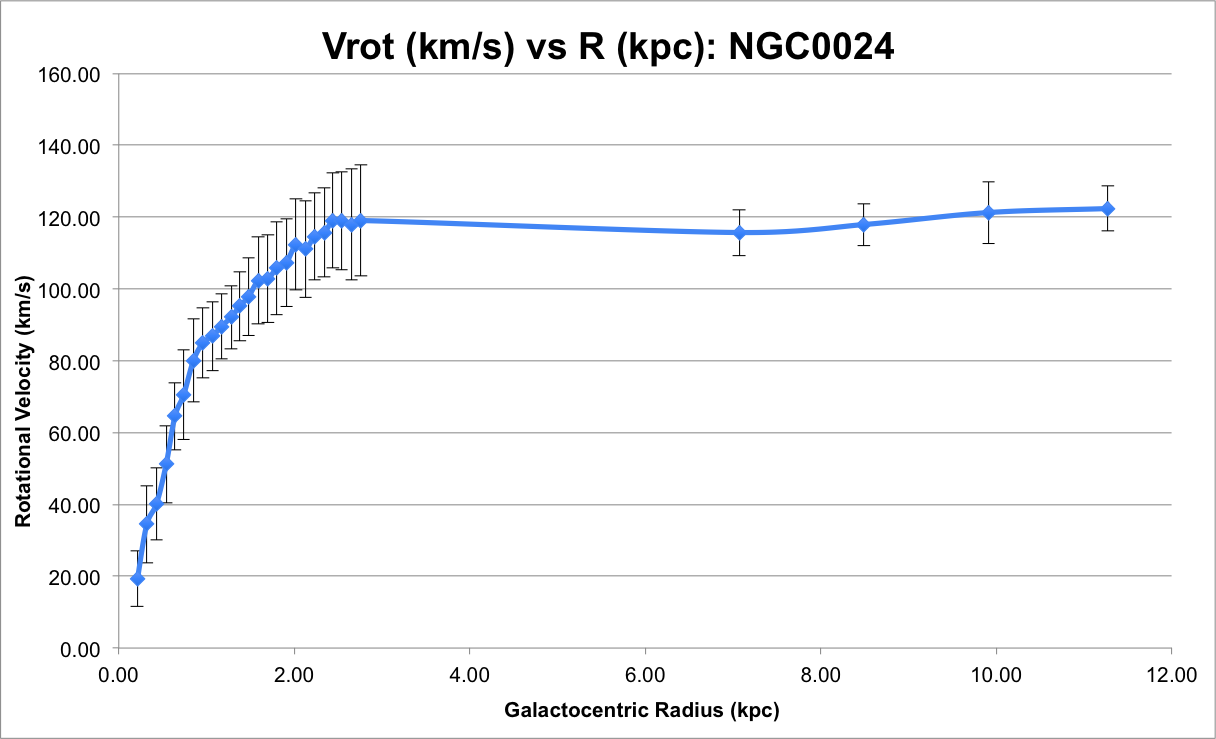
\includegraphics[width=\textwidth]{vrot/Vrot-1}
        \caption{Rotation curve}
    \end{subfigure}
    \hfill
    \begin{subfigure}{0.4\textwidth}
        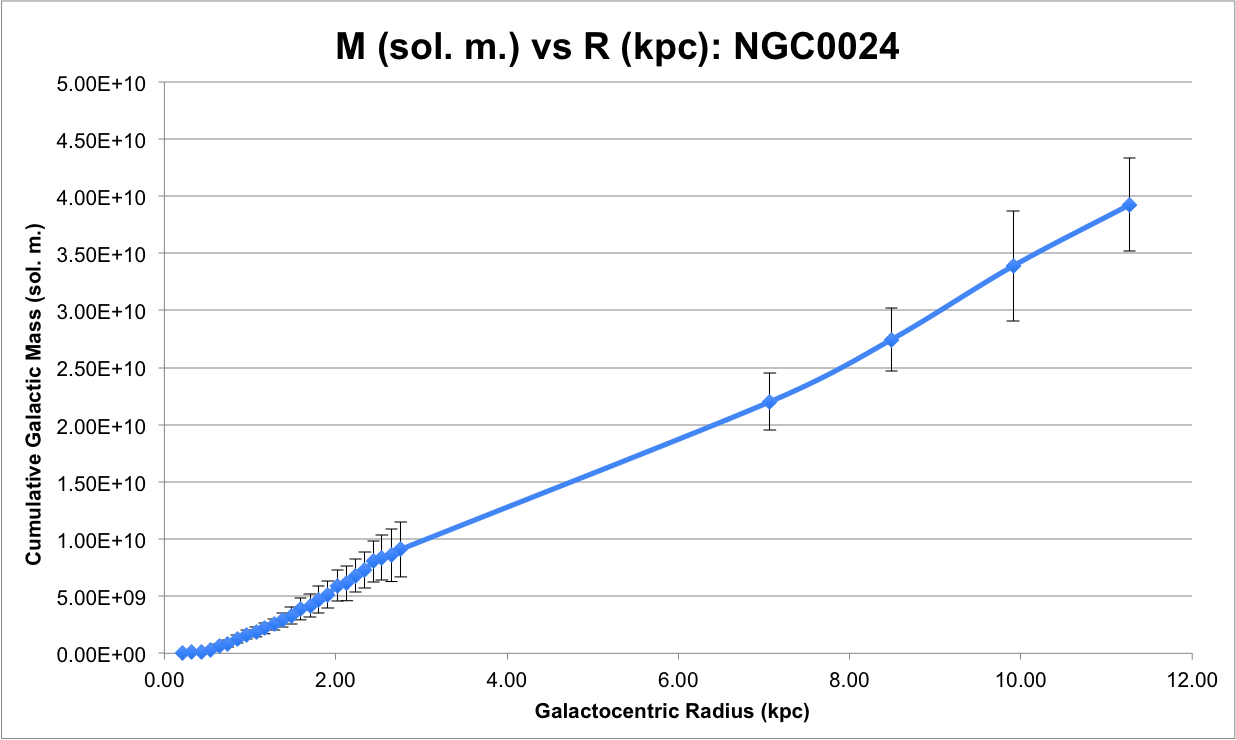
\includegraphics[width=\textwidth]{m/M-1}
        \caption{Cumulative mass distribution}
    \end{subfigure}
    \caption{Rotation curve and cumulative mass distribution for NGC0024.}
    \label{fig:ngc0024}
\end{figure}

\begin{figure}
    \centering
    \begin{subfigure}{0.4\textwidth}
        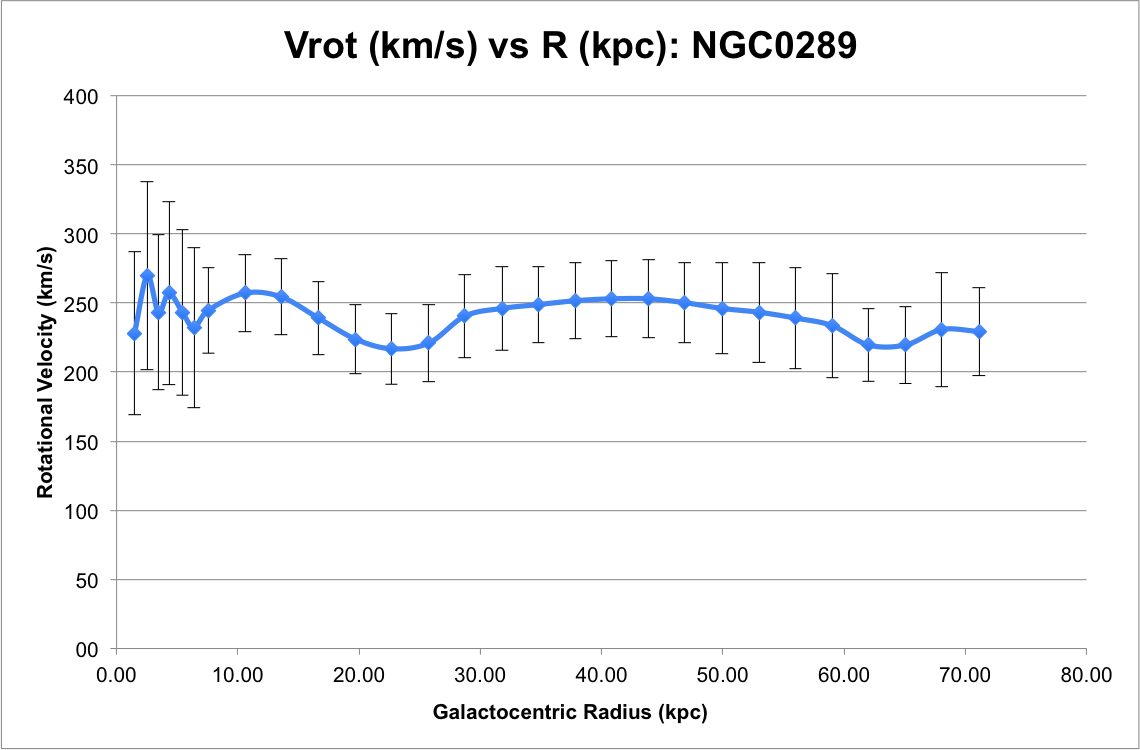
\includegraphics[width=\textwidth]{vrot/Vrot-2}
        \caption{Rotation curve}
    \end{subfigure}
    \hfill
    \begin{subfigure}{0.4\textwidth}
        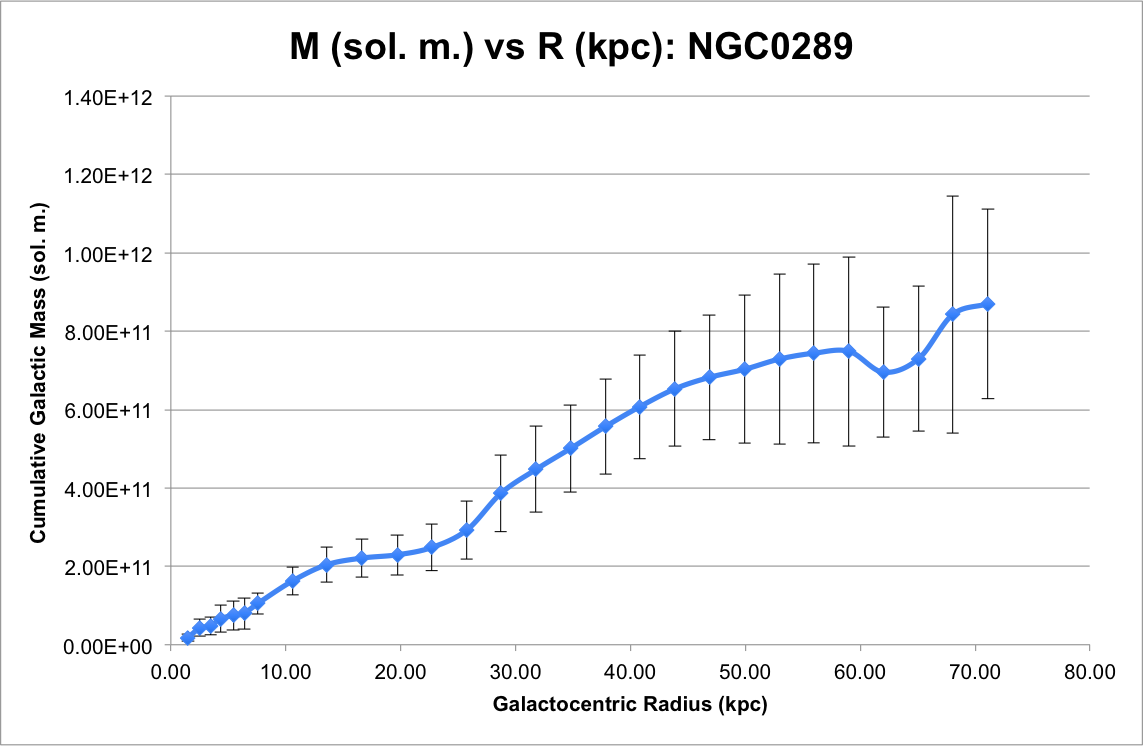
\includegraphics[width=\textwidth]{m/M-2}
        \caption{Cumulative mass distribution}
    \end{subfigure}
    \caption{Rotation curve and cumulative mass distribution for NGC0289.}
    \label{fig:ngc0289}
\end{figure}

\begin{figure}
    \centering
    \begin{subfigure}{0.4\textwidth}
        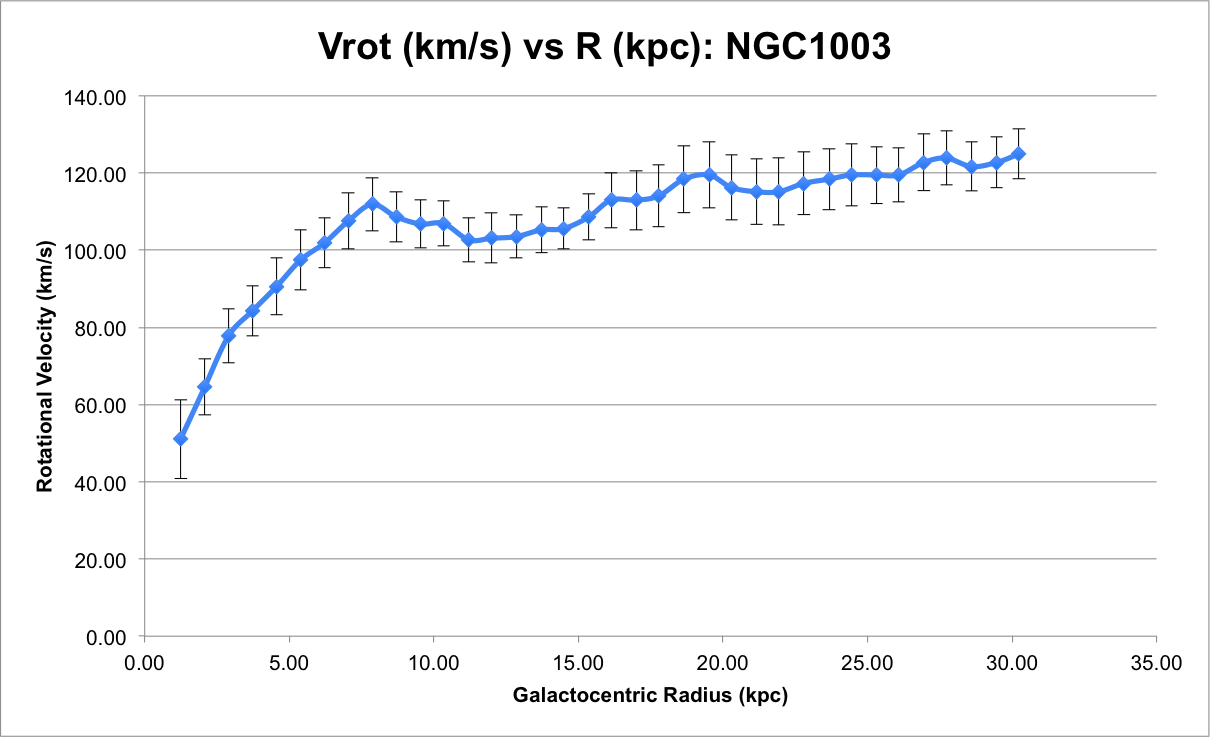
\includegraphics[width=\textwidth]{vrot/Vrot-3}
        \caption{Rotation curve}
    \end{subfigure}
    \hfill
    \begin{subfigure}{0.4\textwidth}
        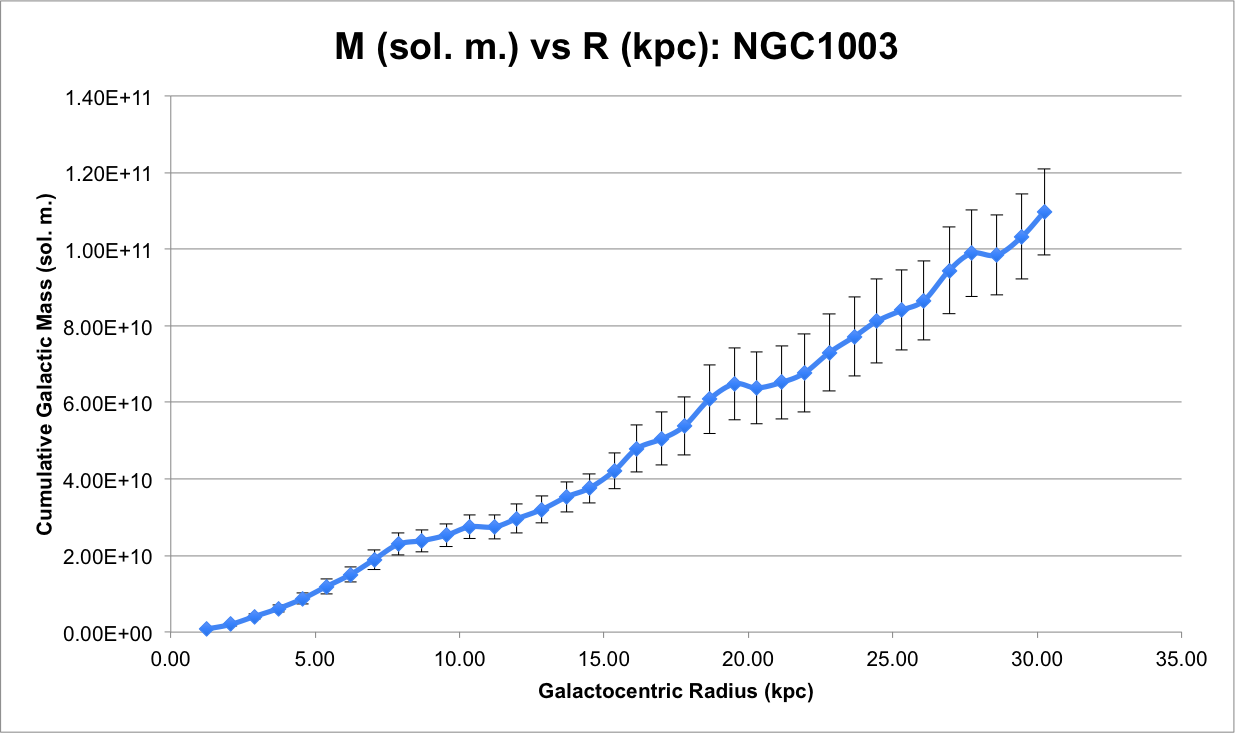
\includegraphics[width=\textwidth]{m/M-3}
        \caption{Cumulative mass distribution}
    \end{subfigure}
    \caption{Rotation curve and cumulative mass distribution for NGC1003.}
    \label{fig:ngc1003}
\end{figure}

\begin{figure}
    \centering
    \begin{subfigure}{0.4\textwidth}
        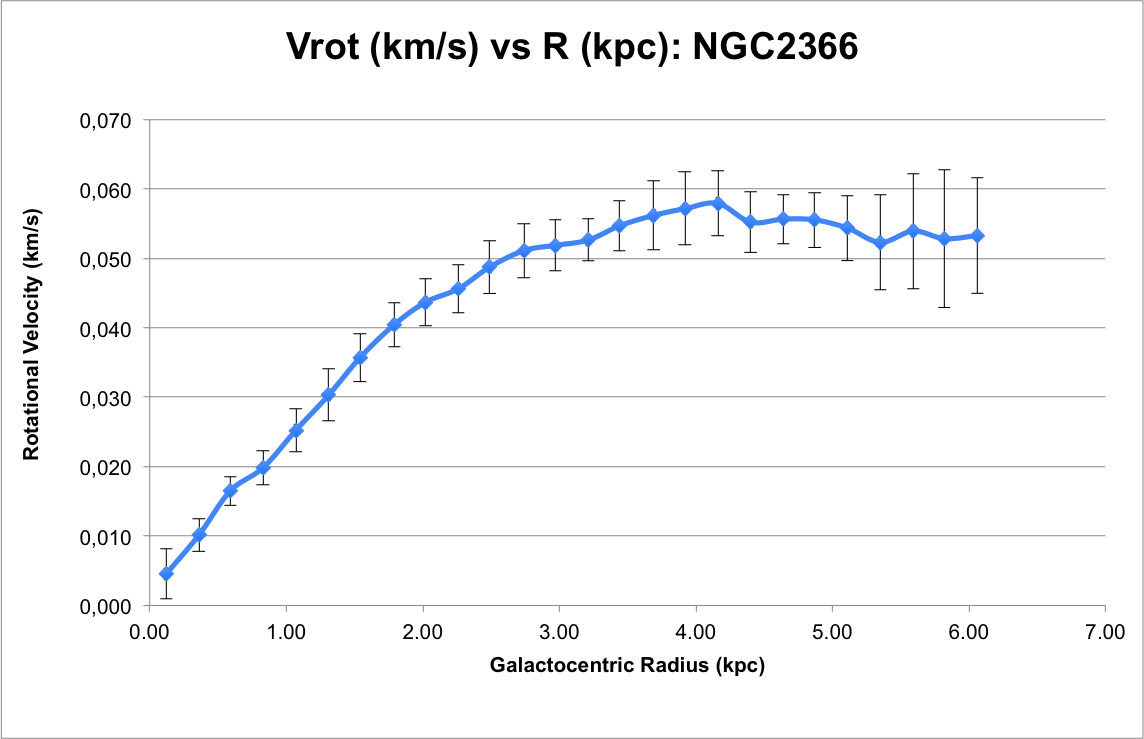
\includegraphics[width=\textwidth]{vrot/Vrot-4}
        \caption{Rotation curve}
    \end{subfigure}
    \hfill
    \begin{subfigure}{0.4\textwidth}
        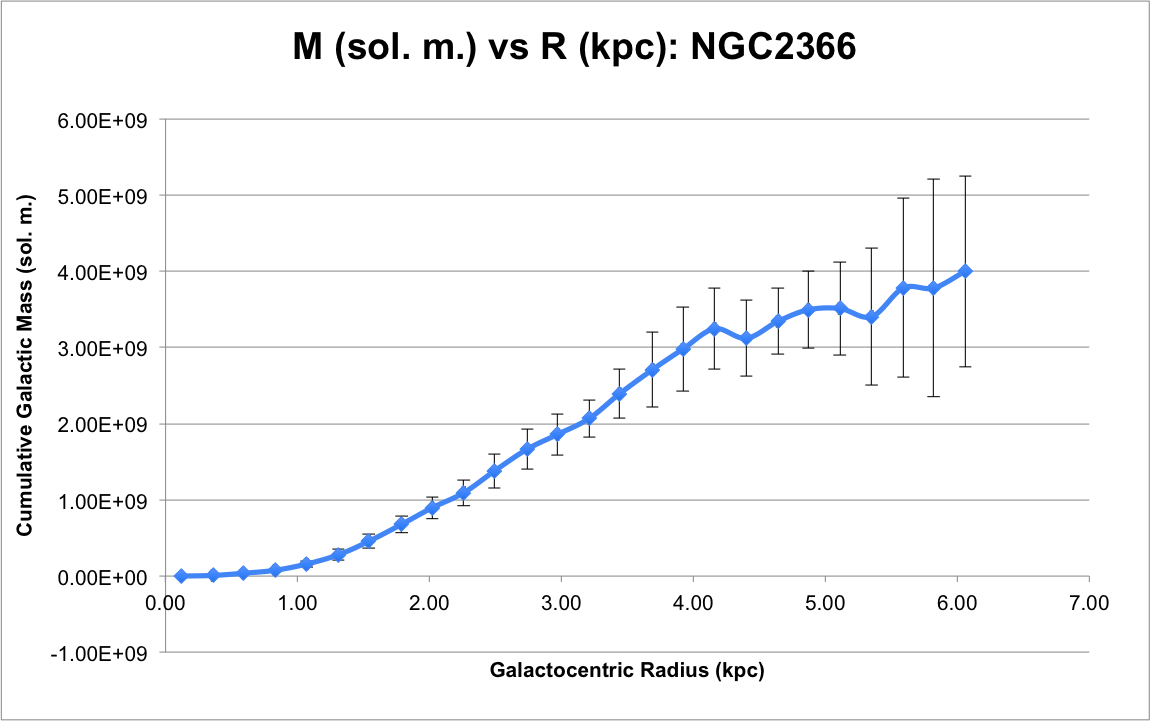
\includegraphics[width=\textwidth]{m/M-4}
        \caption{Cumulative mass distribution}
    \end{subfigure}
    \caption{Rotation curve and cumulative mass distribution for NGC2366.}
    \label{fig:ngc2366}
\end{figure}

\begin{figure}
    \centering
    \begin{subfigure}{0.4\textwidth}
        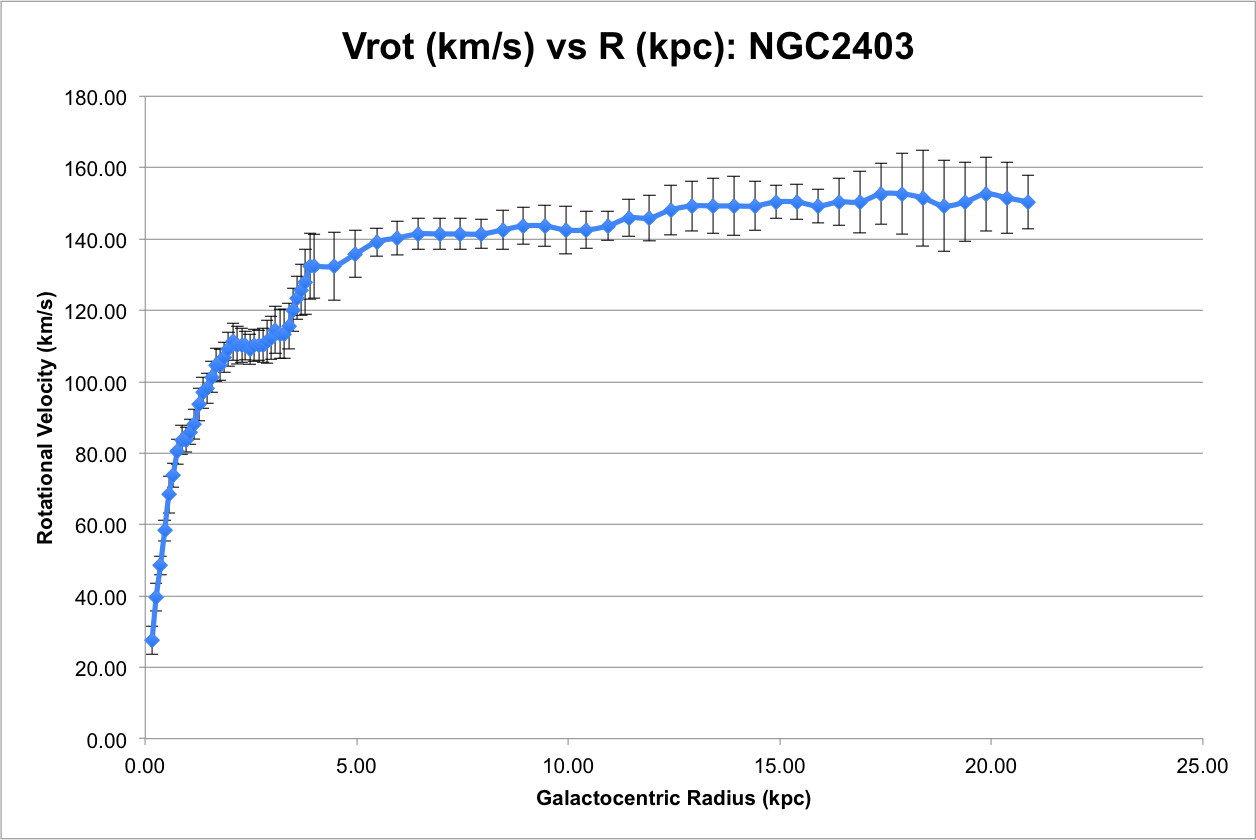
\includegraphics[width=\textwidth]{vrot/Vrot-5}
        \caption{Rotation curve}
    \end{subfigure}
    \hfill
    \begin{subfigure}{0.4\textwidth}
        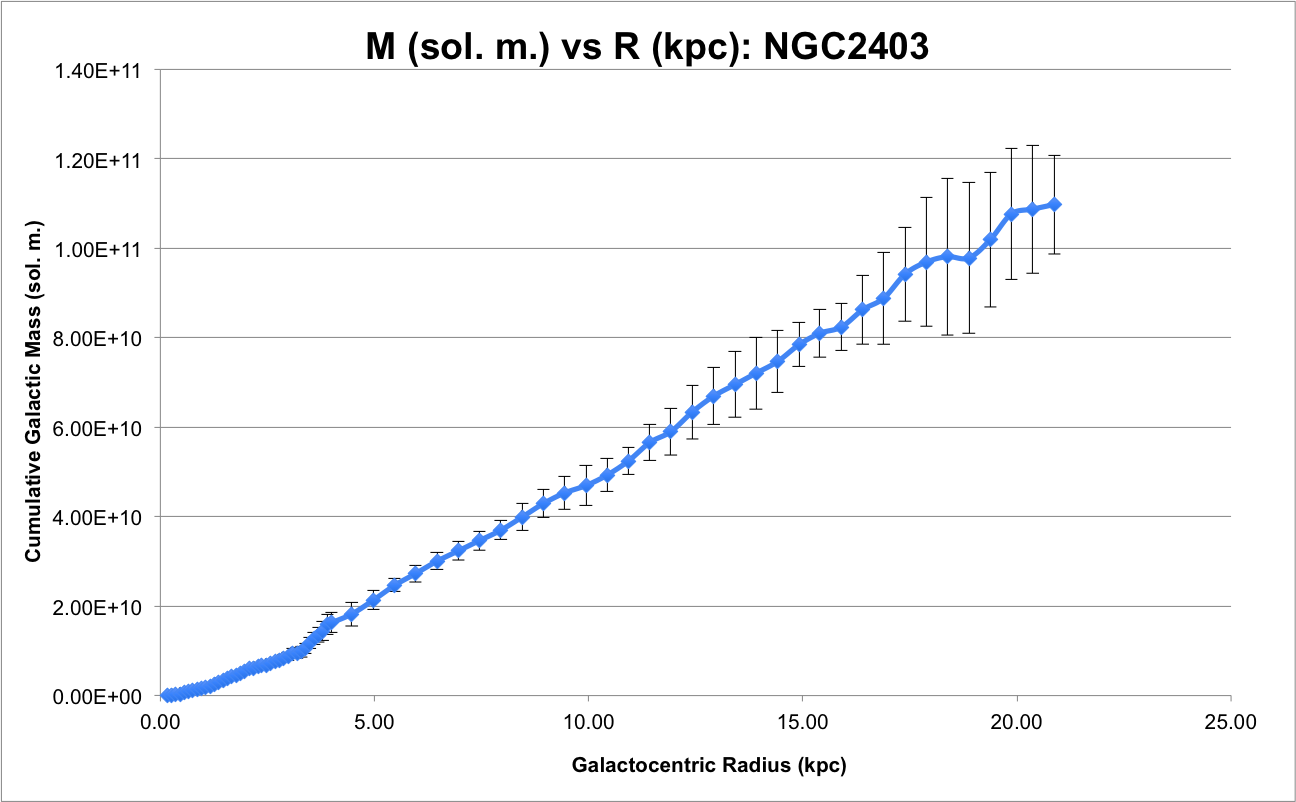
\includegraphics[width=\textwidth]{m/M-5}
        \caption{Cumulative mass distribution}
    \end{subfigure}
    \caption{Rotation curve and cumulative mass distribution for NGC2403.}
    \label{fig:ngc2403}
\end{figure}

\section{Analysis}\label{sec:analysis}

There is an immediate discrepancy between \Cref{fig:expectedgraphs} and \Cref{fig:ngc0024,fig:ngc0289,fig:ngc1003,fig:ngc2366,fig:ngc2403}: for none of the chosen galaxies does the rotation curve fall off according to \Cref{eq:vrotdense} at the boundary of the visible disc.
The radius of NGC2366 is \(8.35/2 = 4.175\,\kpc\) according to \Cref{tab:diameters-inclinations}, for example, and we find in \Cref{tab:proc1003-2366} that after \(r = 4.16\,\kpc\), the corresponding values of \(\vrot\) remaining roughly constant around \(\vrot = 54\,\kmps\); according to \Cref{eq:vrotdense} and \Cref{fig:expectedgraphs}, however, the graph should have decreased according to \(r^{-1/2}\) after this point.
This can be observed in the case of NGC2403 also, on which we have the greatest number of data points.
The radius of NGC2403 is \(27.69/2 = 13.855\,\kpc\) and we see in \Cref{fig:ngc2403} that \(\vrot\) stays very close to \(150\,\kmps\) for nearly \(10\,\kpc\) after this point.
The reason for the rotation curve decreasing after the boundary of the visible disc is that after the visible disc, there is, by definition, no matter that can emit light; otherwise we would have detected it and the radius of the visible disc would have been larger.
This discrepancy in the expected rotation curve and the actual ones suggests that there is still matter outside the visible disc, necessarily unable to emit light, that contributes to an orbital velocity around the galaxy.

The discrepancy in the expected and actual cumulative mass distribution supports this theory.
According to \Cref{fig:expectedgraphs}, the cumulative mass of the galaxy is supposed to stay constant after the end of visible disc, on our assumption that there is no matter outside the visible disc; all the stars of a galaxy, which are the primary contributors to the mass of a galaxy, are located in the visible disc since they emit light.
However, as we see in \Cref{fig:ngc2403}, the cumulative mass of NGC2403 continues to increase even after the end of the visible disc at \(r = 13.855\,\kpc\), that too at seemingly the same rate.
A similar pattern is observed in the other galaxies even after the lack of a large amount of data.
The radius of NGC1003 is \(19.32/2 = 9.66\,\kpc\), for instance, and \Cref{fig:ngc1003} shows a roughly linear continuation of the expected graph after the end of the visible disc for over \(20\,\kpc\).

There are also drops in the cumulative mass at certain points, which should not happen; by definition, cumulative mass always increases and thus drops should never occur.
For example, considering NGC0289, the value of \(M\) decreases from \(7.49\times 10^{11}\,\solmass\) to \(6.95\times 10^{11}\,\solmass\) as \(r\) increases from \(59.03\,\kpc\) to \(62.00\,\kpc\); this drop is quite visible in \Cref{fig:ngc0289}.
Note that the radius of NGC0289 is quite large (\(70.47/2 = 35.235\,\kpc\)) but \(62.00\,\kpc\) is still far beyond the visible disc.
A smaller drop occurs in the case of NGC2366, where \(M\) falls from \(3.51\times 10^9\,\solmass\) to \(3.40\times 10^9\,\solmass\) as \(r\) increases from \(5.11\,\kpc\) to \(5.35\,\kpc\).
In both of these cases, the drop occurs outside of the visible disc.
The values of \(M\) depend on \Cref{eq:internalmass}, and a decrease in \(M\) results from a sufficiently large decrease in \(\vrot\); this is because \(M_i > M_{i+1}\), which means \(r_iv_i^2 > r_{i+1}v_{i+1}^2\), implies
\begin{equation}
    v_{i+1} < \sqrt{\frac{r_i}{r_{i+1}}}v_i.
\end{equation}
Thus two possible explanations arise for this error: either some of the measurements were off --- the observed velocities at these ``drop points'' have been measured to be lower than they actually are, or the inclination measured is higher than the actual inclination --- or \Cref{eq:internalmass} itself is inaccurate, perhaps underlining a limitation of the application of Newton's laws at an astronomical scale.
In any case, since these drops are far and few, and since the rotation curve can generally be described as constant and the cumulative mass distribution linearly increasing after the end of the visible disc, the existence of these drops does not invalidate our conclusions discussed in the next section.

\section{Conclusion}\label{sec:conclusion}

To answer the initial research question, the cumulative mass distribution is linearly increasing for spiral galaxies until well after the end of the visible disc.
Thus, our analysis supports the existence of matter that does not interact with the electromagnetic field but still has mass, in that it imparts gravitational influence like normal luminous matter.
Multiple theories have been proposed for the explanation of this phenomenon.
The most prominent of these is the proposal of the existence of a substance called \textit{dark matter}, which is defined exactly as above: nonluminous matter that still contributes to the gravitational field.
Because of the non-interactivity of dark matter with light, dark matter is very hard to detect \Cite{CERN}, and subsequently there are different theories about the nature of dark matter.
One theory says that dark matter consists of what are called \textit{Weakly Interacting Massive Particles}.
These WIMPs constitute a new proposed elementary particle which interacts through any force that is at least as weak as the weak nuclear force, particularly gravity.
Since WIMPs would be ``invisible'', one strategy used to try to detect them is looking for the theoretical products of reactions that involve them, such as gamma rays or neutrinos.

Another way to answer the dark matter problem was proposed by Israeli physicist Mordehai Milgrom in 1983.
Milgrom hypothesised that the mass discrepancy found in galaxies, such as our own results here, can be explained by opting for a modified version of Newton's law of universal gravitation.
Thus, instead of deducing from the data exhibiting this mass discrepancy that there exists such a thing as ``dark matter'', Milgrom instead argued that the issue arose from the equations used to process the data; Newton's law is not accurate enough to be applied to such galactic phenomena.
Any theory that dare deviate too much from the existing paradigm is heavily criticised, and so was the case with Milgrom too; many physicists are strongly against the idea of modifying classical mechanics and prefer to edit their theories regarding the nature of dark matter.
More importantly, according to other physicists, Milgrom's \textit{MOdified Newtonian Dynamics (MOND)} does not completely remove the need for dark matter since a mass discrepancy in galaxy clusters still persists after MOND considerations.

In any case, research is still being conducted on both dark matter and MOND and we are far from ascertaining the true nature of this unaccounted-for mass.

\section{Evaluation}\label{sec:evaluation}

\begin{itemize}
    \item Why constant uncertainty in \(r\)? (Data given to two decimal places.)
    \item Uncertainty in \(\theta\).
    \item Uncertainties in \(\vobs\) and \(\vrot\).
    \item Uncertainty in \(M\) increases as \(r\) increases.
\end{itemize}

\begin{itemize}
    \item Where does uncertainty come from?
    \item How does this uncertainty affect the conclusion?
\end{itemize}

\appendix

\section{Appendix}

\subsection{Raw Data}\label{sec:raw-data}

% Lorem ipsum dolor sit amet, consectetur adipiscing elit. Praesent mattis, nibh ut venenatis maximus, nibh ex finibus libero, sed fermentum lorem ex ut erat. Proin quis risus vel velit scelerisque laoreet. Maecenas ut eros mattis turpis tincidunt scelerisque quis ut augue. Sed viverra sem eu enim viverra facilisis. Etiam laoreet felis ac dolor malesuada tincidunt. Morbi id ante mauris. Sed laoreet aliquet ante. Interdum et malesuada fames ac ante ipsum primis in faucibus. Fusce leo diam, varius posuere dignissim sit amet, volutpat eu est. Aliquam erat volutpat. Maecenas tincidunt leo elit, mollis dignissim turpis malesuada ut. Ut congue sollicitudin scelerisque. Maecenas sed lectus eu nibh accumsan auctor in dictum tellus.

% \rowcolors{2}{gray!10}{gray!40} % For alternate row-coloring

\singlespacing % Otherwise it gets all wonky
\begin{table}[h!]
    \centering
    \begin{tabular}{|c|c|c|}
        \hline
        Galaxy & Diameter ($\kpc$) & Inclination ($^\circ$) \\
        \hline
        NGC0024 & $19.32$ & $64.0 \pm 3.0$ \\
        NGC0289 & $70.47$ & $46.0 \pm 5.0$ \\
        NGC1003 & $19.32$ & $67.0 \pm 5.0$ \\
        NGC2366 & $8.35$ & $68.0 \pm 5.0$ \\
        NGC2403 & $27.69$ & $63.0 \pm 3.0$ \\ 
        \hline
    \end{tabular}
    \caption{Diameters (NASA) and inclinations (SPARC).}
    \label{tab:diameters-inclinations}
\end{table}
\doublespacing

% Lorem ipsum dolor sit amet, consectetur adipiscing elit. Praesent mattis, nibh ut venenatis maximus, nibh ex finibus libero, sed fermentum lorem ex ut erat. Proin quis risus vel velit scelerisque laoreet. Maecenas ut eros mattis turpis tincidunt scelerisque quis ut augue. Sed viverra sem eu enim viverra facilisis. Etiam laoreet felis ac dolor malesuada tincidunt. Morbi id ante mauris. Sed laoreet aliquet ante. Interdum et malesuada fames ac ante ipsum primis in faucibus. Fusce leo diam, varius posuere dignissim sit amet, volutpat eu est. Aliquam erat volutpat. Maecenas tincidunt leo elit, mollis dignissim turpis malesuada ut. Ut congue sollicitudin scelerisque. Maecenas sed lectus eu nibh accumsan auctor in dictum tellus.

\singlespacing

\begin{table}[h!]
    \begin{tabular}{|c|c|}
        \hline
        \multicolumn{2}{|c|}{NGC0024} \\
        \hline
        $r$ ($\kpc \pm 0.01 \,\kpc$) & $\vobs$ ($\kmps$) \\
        \hline
        $0.21$ & $17.40 \pm 6.51$ \\
        $0.32$ & $31.00 \pm 8.86$ \\
        $0.43$ & $36.10 \pm 8.16$ \\
        $0.54$ & $46.00 \pm 8.52$ \\
        $0.64$ & $58.00 \pm 6.90$ \\
        $0.74$ & $63.40 \pm 9.55$ \\
        $0.85$ & $71.90 \pm 8.52$ \\
        $0.96$ & $76.40 \pm 6.82$ \\
        $1.07$ & $78.10 \pm 6.65$ \\
        $1.17$ & $80.50 \pm 6.14$ \\
        $1.28$ & $82.80 \pm 5.80$ \\
        $1.38$ & $85.60 \pm 6.48$ \\
        $1.48$ & $88.00 \pm 7.50$ \\
        $1.59$ & $92.00 \pm 8.52$ \\
        $1.70$ & $92.40 \pm 8.52$ \\
        $1.80$ & $95.10 \pm 9.20$ \\
        $1.91$ & $96.50 \pm 8.52$ \\
        $2.02$ & $101.00 \pm 8.86$ \\
        $2.13$ & $99.90 \pm 9.55$ \\
        $2.23$ & $103.00 \pm 8.18$ \\
        $2.34$ & $104.00 \pm 8.52$ \\
        $2.44$ & $107.00 \pm 9.20$ \\
        $2.54$ & $107.00 \pm 9.55$ \\
        $2.65$ & $106.00 \pm 11.20$ \\
        $2.76$ & $107.00 \pm 11.20$ \\
        $7.07$ & $104.00 \pm 3.11$ \\
        $8.49$ & $106.00 \pm 2.55$ \\
        $9.91$ & $109.00 \pm 4.95$ \\
        $11.27$ & $110.00 \pm 2.83$ \\
        \hline
    \end{tabular}
    \hfill
    \begin{tabular}{|c|c|}
        \hline
        \multicolumn{2}{|c|}{NGC0289} \\
        \hline
        $r$ ($\kpc \pm 0.01 \,\kpc$) & $\vobs$ ($\kmps$) \\
        \hline
        $1.50$ & $164.00 \pm 28.20$ \\
        $2.52$ & $194.00 \pm 32.00$ \\
        $3.46$ & $175.00 \pm 25.20$ \\
        $4.32$ & $185.00 \pm 31.50$ \\
        $5.43$ & $175.00 \pm 27.90$ \\
        $6.38$ & $167.00 \pm 27.20$ \\
        $7.57$ & $176.00 \pm 7.18$ \\
        $10.60$ & $185.00 \pm 4.29$ \\
        $13.57$ & $183.00 \pm 4.22$ \\
        $16.64$ & $172.00 \pm 4.33$ \\
        $19.71$ & $161.00 \pm 4.24$ \\
        $22.68$ & $156.00 \pm 5.08$ \\
        $25.75$ & $159.00 \pm 6.49$ \\
        $28.72$ & $173.00 \pm 6.97$ \\
        $31.79$ & $177.00 \pm 6.57$ \\
        $34.77$ & $179.00 \pm 4.47$ \\
        $37.84$ & $181.00 \pm 4.26$ \\
        $40.81$ & $182.00 \pm 4.26$ \\
        $43.88$ & $182.00 \pm 4.83$ \\
        $46.85$ & $180.00 \pm 5.50$ \\
        $49.92$ & $177.00 \pm 8.50$ \\
        $52.99$ & $175.00 \pm 11.00$ \\
        $55.96$ & $172.00 \pm 11.60$ \\
        $59.03$ & $168.00 \pm 12.60$ \\
        $62.00$ & $158.00 \pm 5.38$ \\
        $65.07$ & $158.00 \pm 6.50$ \\
        $68.05$ & $166.00 \pm 15.50$ \\
        $71.12$ & $165.00 \pm 8.75$ \\
        \hline
    \end{tabular}
    \caption{$\vobs$ data for NGC0024 and NGC0289 (SPARC).}
    \label{tab:raw0024-0289}
\end{table}

\begin{table}[h!]
    \begin{tabular}{|c|c|}
        \hline
        \multicolumn{2}{|c|}{NGC1003} \\
        \hline
        $r$ ($\kpc \pm 0.01 \,\kpc$) & $\vobs$ ($\kmps$) \\
        \hline
        $1.25$ & $47.00 \pm 7.60$ \\
        $2.08$ & $59.50 \pm 4.50$ \\
        $2.90$ & $71.60 \pm 3.70$ \\
        $3.73$ & $77.60 \pm 3.10$ \\
        $4.56$ & $83.40 \pm 3.60$ \\
        $5.39$ & $89.70 \pm 3.80$ \\
        $6.22$ & $93.80 \pm 2.40$ \\
        $7.04$ & $99.00 \pm 3.00$ \\
        $7.87$ & $103.00 \pm 2.50$ \\
        $8.70$ & $100.00 \pm 2.30$ \\
        $9.54$ & $98.30 \pm 2.00$ \\
        $10.34$ & $98.40 \pm 1.70$ \\
        $11.21$ & $94.50 \pm 1.80$ \\
        $11.98$ & $94.90 \pm 2.40$ \\
        $12.85$ & $95.30 \pm 1.60$ \\
        $13.72$ & $96.90 \pm 1.80$ \\
        $14.49$ & $97.20 \pm 1.30$ \\
        $15.36$ & $100.00 \pm 1.80$ \\
        $16.13$ & $104.00 \pm 2.70$ \\
        $17.00$ & $104.00 \pm 3.20$ \\
        $17.78$ & $105.00 \pm 3.40$ \\
        $18.65$ & $109.00 \pm 3.90$ \\
        $19.52$ & $110.00 \pm 3.80$ \\
        $20.29$ & $107.00 \pm 3.80$ \\
        $21.16$ & $106.00 \pm 3.80$ \\
        $21.93$ & $106.00 \pm 4.00$ \\
        $22.80$ & $108.00 \pm 3.40$ \\
        $23.67$ & $109.00 \pm 3.20$ \\
        $24.44$ & $110.00 \pm 3.30$ \\
        $25.31$ & $110.00 \pm 2.70$ \\
        $26.08$ & $110.00 \pm 2.40$ \\
        $26.95$ & $113.00 \pm 2.50$ \\
        $27.73$ & $114.00 \pm 2.20$ \\
        $28.60$ & $112.00 \pm 1.70$ \\
        $29.47$ & $113.00 \pm 1.80$ \\
        $30.24$ & $115.00 \pm 1.60$ \\
        \hline
    \end{tabular}
    \hfill
    \begin{tabular}{|c|c|}
        \hline
        \multicolumn{2}{|c|}{NGC2366} \\
        \hline
        $r$ ($\kpc \pm 0.01 \,\kpc$) & $\vobs$ ($\kmps$) \\
        \hline
        $0.12$ & $4.20 \pm 3.15$ \\
        $0.36$ & $9.41 \pm 1.83$ \\
        $0.59$ & $15.30 \pm 1.37$ \\
        $0.83$ & $18.40 \pm 1.64$ \\
        $1.07$ & $23.40 \pm 2.08$ \\
        $1.31$ & $28.10 \pm 2.46$ \\
        $1.54$ & $33.10 \pm 2.01$ \\
        $1.79$ & $37.50 \pm 1.62$ \\
        $2.02$ & $40.50 \pm 1.68$ \\
        $2.26$ & $42.30 \pm 1.69$ \\
        $2.49$ & $45.20 \pm 1.91$ \\
        $2.74$ & $47.40 \pm 1.95$ \\
        $2.97$ & $48.10 \pm 1.74$ \\
        $3.21$ & $48.80 \pm 1.08$ \\
        $3.44$ & $50.70 \pm 1.55$ \\
        $3.69$ & $52.10 \pm 2.78$ \\
        $3.92$ & $53.00 \pm 2.98$ \\
        $4.16$ & $53.70 \pm 2.39$ \\
        $4.40$ & $51.20 \pm 2.21$ \\
        $4.64$ & $51.60 \pm 1.45$ \\
        $4.87$ & $51.50 \pm 1.84$ \\
        $5.11$ & $50.40 \pm 2.53$ \\
        $5.35$ & $48.50 \pm 4.60$ \\
        $5.59$ & $50.00 \pm 5.91$ \\
        $5.82$ & $49.00 \pm 7.42$ \\
        $6.06$ & $49.40 \pm 5.92$ \\
        \hline
    \end{tabular}
    \caption{$\vobs$ data for NGC1003 and NGC2366 (SPARC).}
    \label{tab:raw1003-2366}
\end{table}

\begin{table}[h!]
    \begin{tabular}{|c|c|}
        \hline
        \multicolumn{2}{|c|}{NGC2403} \\
        \hline
        $r$ ($\kpc \pm 0.01 \,\kpc$) & $\vobs$ ($\kmps$) \\
        \hline
        $0.16$ & $24.50 \pm 2.83$ \\
        $0.26$ & $35.30 \pm 2.46$ \\
        $0.36$ & $43.20 \pm 1.12$ \\
        $0.46$ & $52.00 \pm 1.25$ \\
        $0.56$ & $60.90 \pm 2.93$ \\
        $0.66$ & $65.80 \pm 1.25$ \\
        $0.76$ & $71.70 \pm 1.25$ \\
        $0.86$ & $74.60 \pm 1.60$ \\
        $0.96$ & $74.60 \pm 1.03$ \\
        $1.06$ & $76.60 \pm 1.12$ \\
        $1.16$ & $78.50 \pm 1.60$ \\
        $1.27$ & $83.40 \pm 1.80$ \\
        $1.36$ & $86.40 \pm 1.60$ \\
        $1.47$ & $87.40 \pm 1.41$ \\
        $1.57$ & $90.30 \pm 1.41$ \\
        $1.67$ & $93.30 \pm 1.60$ \\
        $1.77$ & $93.30 \pm 1.41$ \\
        $1.87$ & $95.20 \pm 1.25$ \\
        $1.97$ & $97.20 \pm 1.60$ \\
        $2.08$ & $99.10 \pm 2.02$ \\
        $2.18$ & $98.20 \pm 2.02$ \\
        $2.28$ & $98.20 \pm 1.60$ \\
        $2.37$ & $98.20 \pm 1.00$ \\
        $2.47$ & $97.20 \pm 1.12$ \\
        $2.57$ & $98.20 \pm 1.41$ \\
        $2.68$ & $98.20 \pm 1.12$ \\
        $2.78$ & $98.20 \pm 1.60$ \\
        $2.88$ & $99.10 \pm 2.69$ \\
        $2.98$ & $100.00 \pm 2.69$ \\
        $3.08$ & $102.00 \pm 3.16$ \\
        $3.19$ & $101.00 \pm 3.40$ \\
        $3.29$ & $101.00 \pm 3.40$ \\
        $3.39$ & $103.00 \pm 2.93$ \\
        $3.49$ & $107.00 \pm 2.46$ \\
        $3.59$ & $110.00 \pm 2.46$ \\
        $3.69$ & $112.00 \pm 3.40$ \\
        $3.79$ & $114.00 \pm 5.10$ \\
        $3.90$ & $118.00 \pm 5.10$ \\
        \hline
    \end{tabular}
    \hfill
    \begin{tabular}{|c|c|}
        \hline
        $r$ ($\kpc \pm 0.01 \,\kpc$) & $\vobs$ ($\kmps$) \\
        \hline
        $3.99$ & $118.00 \pm 4.85$ \\
        $4.47$ & $118.00 \pm 5.36$ \\
        $4.97$ & $121.00 \pm 2.57$ \\
        $5.47$ & $124.00 \pm 0.22$ \\
        $5.96$ & $125.00 \pm 0.88$ \\
        $6.46$ & $126.00 \pm 0.45$ \\
        $6.96$ & $126.00 \pm 0.55$ \\
        $7.45$ & $126.00 \pm 0.45$ \\
        $7.95$ & $126.00 \pm 0.24$ \\
        $8.45$ & $127.00 \pm 1.45$ \\
        $8.94$ & $128.00 \pm 1.12$ \\
        $9.44$ & $128.00 \pm 1.68$ \\
        $9.94$ & $127.00 \pm 2.56$ \\
        $10.43$ & $127.00 \pm 1.24$ \\
        $10.93$ & $128.00 \pm 0.21$ \\
        $11.43$ & $130.00 \pm 1.13$ \\
        $11.92$ & $130.00 \pm 2.23$ \\
        $12.42$ & $132.00 \pm 2.68$ \\
        $12.92$ & $133.00 \pm 2.68$ \\
        $13.42$ & $133.00 \pm 3.37$ \\
        $13.91$ & $133.00 \pm 3.81$ \\
        $14.41$ & $133.00 \pm 2.56$ \\
        $14.91$ & $134.00 \pm 0.56$ \\
        $15.40$ & $134.00 \pm 0.79$ \\
        $15.90$ & $133.00 \pm 0.67$ \\
        $16.40$ & $134.00 \pm 2.35$ \\
        $16.89$ & $134.00 \pm 4.13$ \\
        $17.39$ & $136.00 \pm 3.91$ \\
        $17.89$ & $136.00 \pm 6.38$ \\
        $18.38$ & $135.00 \pm 8.39$ \\
        $18.88$ & $133.00 \pm 7.83$ \\
        $19.38$ & $134.00 \pm 6.26$ \\
        $19.87$ & $136.00 \pm 5.60$ \\
        $20.37$ & $135.00 \pm 5.24$ \\
        $20.87$ & $134.00 \pm 3.12$ \\
        \hline
    \end{tabular}
    \caption{$\vobs$ data for NGC2403 (SPARC).}
    \label{tab:raw2403}
\end{table}

\doublespacing

\nocite{*}
\printbibliography

\end{document}
